% !TeX program = pdfLaTeX
\documentclass[12pt]{article}
\usepackage{amsmath}
\usepackage{graphicx,psfrag,epsf}
\usepackage{enumerate}
\usepackage{natbib}
\usepackage{textcomp}
\usepackage[hyphens]{url} % not crucial - just used below for the URL
\usepackage{hyperref}
\providecommand{\tightlist}{%
  \setlength{\itemsep}{0pt}\setlength{\parskip}{0pt}}

%\pdfminorversion=4
% NOTE: To produce blinded version, replace "0" with "1" below.
\newcommand{\blind}{0}

% DON'T change margins - should be 1 inch all around.
\addtolength{\oddsidemargin}{-.5in}%
\addtolength{\evensidemargin}{-.5in}%
\addtolength{\textwidth}{1in}%
\addtolength{\textheight}{1.3in}%
\addtolength{\topmargin}{-.8in}%

%% load any required packages here



% Pandoc citation processing
\newlength{\csllabelwidth}
\setlength{\csllabelwidth}{3em}
\newlength{\cslhangindent}
\setlength{\cslhangindent}{1.5em}
% for Pandoc 2.8 to 2.10.1
\newenvironment{cslreferences}%
  {}%
  {\par}
% For Pandoc 2.11+
\newenvironment{CSLReferences}[3] % #1 hanging-ident, #2 entry spacing
 {% don't indent paragraphs
  \setlength{\parindent}{0pt}
  % turn on hanging indent if param 1 is 1
  \ifodd #1 \everypar{\setlength{\hangindent}{\cslhangindent}}\ignorespaces\fi
  % set entry spacing
  \ifnum #2 > 0
  \setlength{\parskip}{#2\baselineskip}
  \fi
 }%
 {}
\usepackage{calc} % for calculating minipage widths
\newcommand{\CSLBlock}[1]{#1\hfill\break}
\newcommand{\CSLLeftMargin}[1]{\parbox[t]{\csllabelwidth}{#1}}
\newcommand{\CSLRightInline}[1]{\parbox[t]{\linewidth - \csllabelwidth}{#1}}
\newcommand{\CSLIndent}[1]{\hspace{\cslhangindent}#1}

%% Any special functions or other packages can be loaded here.
\usepackage[utf8]{inputenc}
\usepackage[flushleft]{threeparttable}
\usepackage{multirow}
\usepackage[normalem]{ulem}
\useunder{\uline}{\ul}{}
%% \usepackage{makecell,interfaces-makecell} %latex error
\usepackage[]{graphicx}
\usepackage[]{color}
\usepackage{xcolor}
% \usepackage[ruled,vlined,linesnumbered]{algorithm2e}
\usepackage{algorithmic}
\usepackage{bm}
\usepackage{etoolbox}
\usepackage{tabu}
\usepackage{placeins}
\setlength {\marginparwidth }{2cm}
\usepackage{todonotes}
\urlstyle{tt}  % don't use monospace font for urls
\allowdisplaybreaks


\usepackage[ruled,vlined,linesnumbered]{algorithm2e}
\usepackage{amsmath, amsfonts, amssymb, bm, mathtools, todonotes, booktabs, microtype}

\makeatletter
%If bera loaded, this is monash wp.
\@ifpackageloaded{bera}{}{\usepackage{mathptmx}}
\makeatother
\usepackage[cal = txupr]{mathalpha}


\makeatletter
\@ifpackageloaded{geometry}{}{\usepackage{geometry}}
\makeatother
\geometry{margin=2.2cm}

\mathtoolsset{showonlyrefs}
\newcommand{\argmax}{\mathop{\text{arg\,max}}}
\clubpenalty = 10000
\widowpenalty = 10000
\brokenpenalty = 10000
\usepackage{graphicx}
\setcounter{topnumber}{2}
\setcounter{bottomnumber}{2}
\setcounter{totalnumber}{4}
\renewcommand{\topfraction}{0.9}
\renewcommand{\bottomfraction}{0.9}
\renewcommand{\textfraction}{0.1}
\renewcommand{\floatpagefraction}{0.9}

\usepackage{caption}
\DeclareCaptionStyle{italic}[justification=centering]
 {labelfont={bf},textfont={it},labelsep=colon}
\captionsetup[figure]{style=italic,format=hang,singlelinecheck=true}
\captionsetup[table]{style=italic,format=hang,singlelinecheck=true}


\begin{document}


\def\spacingset#1{\renewcommand{\baselinestretch}%
{#1}\small\normalsize} \spacingset{1}


%%%%%%%%%%%%%%%%%%%%%%%%%%%%%%%%%%%%%%%%%%%%%%%%%%%%%%%%%%%%%%%%%%%%%%%%%%%%%%

\if0\blind
{
  \title{\bf Manifold learning with approximate nearest neighbors}

  \author{
        Fan Cheng \thanks{\href{mailto:Fan.Cheng@monash.edu}{\nolinkurl{Fan.Cheng@monash.edu}}} \\
    Monash University\\
     and \\     Rob J Hyndman \\
    Monash University\\
     and \\     Anastasios Panagiotelis \\
    University of Sydney\\
      }
  \maketitle
} \fi

\if1\blind
{
  \bigskip
  \bigskip
  \bigskip
  \begin{center}
    {\LARGE\bf Manifold learning with approximate nearest neighbors}
  \end{center}
  \medskip
} \fi

\bigskip
\begin{abstract}
Manifold learning algorithms are valuable tools for the analysis of high-dimensional data, many of which include a step where nearest neighbors of all observations are found. This can present a computational bottleneck when the number of observations is large or when the observations lie in more general metric spaces, such as statistical manifolds, which require all pairwise distances between observations to be computed. We resolve this problem by using a broad range of approximate nearest neighbor algorithms within manifold learning algorithms and evaluating their impact on embedding accuracy. We use approximate nearest neighbors for statistical manifolds by exploiting the connection between Hellinger/Total variation distance for discrete distributions and the L2/L1 norm. Via a thorough empirical investigation based on the benchmark MNIST dataset, it is shown that approximate nearest neighbors lead to substantial improvements in computational time with little to no loss in the accuracy of the embedding produced by a manifold learning algorithm. This result is robust to the use of different manifold learning algorithms, to the use of different approximate nearest neighbor algorithms, and to the use of different measures of embedding accuracy. The proposed method is applied to learning statistical manifolds data on distributions of electricity usage. This application demonstrates how the proposed methods can be used to visualize and identify anomalies and uncover underlying structure within high-dimensional data in a way that is scalable to large datasets.
\end{abstract}

\noindent%
{\it Keywords:} statistical manifold, dimension reduction, anomaly detection, k-d trees, Hellinger distance, smart meter data
\vfill

\newpage
\spacingset{1.45} % DON'T change the spacing!

\newpage

\hypertarget{introduction}{%
\section{Introduction}\label{introduction}}

Modern data often comprise a large number of high-dimensional observations in a possibly non-Euclidean space. Dimension reduction can be an important tool for exploring and analyzing such data for tasks such as clustering, classification, visualization, and anomaly detection. If high-dimensional data are assumed to lie on a lower-dimensional manifold, then
manifold learning algorithms (see \protect\hyperlink{ref-Cayton2005-dp}{Cayton} (\protect\hyperlink{ref-Cayton2005-dp}{2005}), \protect\hyperlink{ref-Lee2007-wq}{J. A. Lee and Verleysen} (\protect\hyperlink{ref-Lee2007-wq}{2007}) and \protect\hyperlink{ref-Izenman2012-mx}{Izenman} (\protect\hyperlink{ref-Izenman2012-mx}{2012}) for reviews) can be used to extract a low dimensional representation of the data. Applications of manifold learning algorithms include analyzing cell characteristics in clinical cell cytometry (\protect\hyperlink{ref-Carter2009-ti}{Carter et al. 2009}), classification and visualization in hyperspectral image analysis (\protect\hyperlink{ref-Lunga2014-kc}{Lunga et al. 2014}), image reconstruction during an MRI acquisition (\protect\hyperlink{ref-Zhu2018-jw}{Zhu et al. 2018}) and detecting anomalous probability distributions of household electricity usage (\protect\hyperlink{ref-Hyndman2018-ia}{R. J. Hyndman, Liu, and Pinson 2018}). The last of these examples pose a number of challenges that provide the motivation for two novel contributions proposed in this manuscript. The first is to consider the use of a wide range of contemporary approximate nearest neighbor methods, as opposed to exact nearest neighbors within manifold learning algorithms, and to thoroughly investigate the effect of this approximation on the accuracy of manifold learning. The second is to incorporate approximate nearest neighbor algorithms into manifold learning for statistical manifolds - that is a manifold whose elements are probability distributions. This is achieved by finding discrete approximations to each distribution and then exploiting the link between Hellinger (or Total Variation) distance and the L2 (or L1) norm.

Linear methods for dimension reduction date at least as far back as the development of Principal Components Analysis, while a number of non-linear methods were developed in the 1960s (\protect\hyperlink{ref-Shepard1962-ac}{Shepard 1962a}, \protect\hyperlink{ref-Shepard1962-ft}{1962b}; \protect\hyperlink{ref-Kruskal1964-iv}{Kruskal 1964a}, \protect\hyperlink{ref-Kruskal1964-md}{1964b}). A further flourishing in the development of non-linear dimension reduction techniques gained traction after ISOMAP (\protect\hyperlink{ref-Tenenbaum2000-fr}{Tenenbaum, Silva, and Langford 2000}) and Local Linear Embedding (LLE) (\protect\hyperlink{ref-Roweis2000-ni}{Roweis and Saul 2000}) were introduced in the same issue of \emph{Science}. These methods assume data lie on a manifold and are hence known as manifold learning techniques. Some algorithms developed in the early 2000s include, but are not limited to, Laplacian eigenmaps (\protect\hyperlink{ref-Belkin2003-kz}{Belkin and Niyogi 2003}), Hessian LLE (\protect\hyperlink{ref-Donoho2003-am}{Donoho and Grimes 2003}), local tangent space alignment (\protect\hyperlink{ref-Zhang2003-yi}{Zhang and Zha 2003}), diffusion maps (\protect\hyperlink{ref-Nadler2006-cm}{Nadler et al. 2006}; \protect\hyperlink{ref-Coifman2006-no}{Coifman and Lafon 2006}), semi-definite embedding (\protect\hyperlink{ref-Weinberger2006-dc}{Weinberger and Saul 2006}), and t-SNE (\protect\hyperlink{ref-Maaten2008-dw}{Maaten and Hinton 2008}). While these algorithms all differ, several contain a common step which is to compute a graph of \(K\)-nearest neighbors. These include ISOMAP, LLE, Laplacian Eigenmaps, and Hessian LLE which are the four manifold learning algorithms we consider in this paper.

Computing \(K\) nearest neighbors can be a significant computational bottleneck especially when the number of observations is large. A naive way to find the nearest neighbors is to compute pairwise distances between all observations - an \(O(N^2)\) operation. For some metrics including Euclidean and Manhattan distance, more efficient solutions that find the \(K\) nearest neighbors in \(O(Nlog(N))\) time are available, for example, k-d trees (\protect\hyperlink{ref-Bentley1975-zo}{Bentley 1975}). Some software implementations of manifold learning techniques, including the R package \emph{dimRed} (\protect\hyperlink{ref-Kraemer2018-zf}{Kraemer, Reichstein, and Mahecha 2018}) exploit such algorithms. For applications with an extremely large number of observations, faster approximate versions of k-d trees can be used for nearest neighbor search. \protect\hyperlink{ref-McQueen2016-xz}{McQueen et al.} (\protect\hyperlink{ref-McQueen2016-xz}{2016}) provides one such implementation through the Python package, \emph{megaman}, which exploits the \emph{FLANN} (\protect\hyperlink{ref-Muja2009-de}{Muja and Lowe 2009}) package for fast neighbor searching\footnote{approximate nearest neighbors using k-d trees can be implemented in R using the C++ ANN library (\protect\hyperlink{ref-mount2010-ann}{Mount and Arya 2010}) is wrapped in the R package \emph{RANN} (\protect\hyperlink{ref-jefferislab2019-l2}{Mount et al. 2019})}. However, to the best of our knowledge, no work has been done on evaluating the effect of using approximate nearest neighbors on the accuracy of embeddings produces by manifold learning algorithms. Furthermore, more recent research on approximate nearest neighbor search has seen alternative and arguably more efficient alternatives to k-d trees emerge, including as Annoy (\protect\hyperlink{ref-Bernhardsson2016-tf}{Spotify 2016}) and Hierarchical Navigable Small Worlds (HNSW) (\protect\hyperlink{ref-Malkov2020-jp}{Malkov and Yashunin 2020}). Consequently, the first main novel contribution in this paper is to thoroughly evaluate the impact of using approximate nearest neighbor search within manifold learning and to compare a broad range of approximate nearest neighbors in doing so.

We evaluate the impact of using approximate nearest neighbor search in manifold learning in two main ways. First, it is important to establish that using ANN algorithms improves, in a substantive manner, the speed of manifold learning algorithms. Via a thorough empirical study using the benchmark MNIST dataset, we establish that in practice, up to a four-fold improvement in computational time can be achieved when using ANN, relative to exact nearest neighbors even if k-d trees are used for the exact solution. The improvements in computational speed are greatest for the Annoy algorithm and for Laplacian Eigenmaps. Second, it is important to establish that using ANN algorithms does not lead to a substantial deterioration in the accuracy of embeddings produced by manifold learning algorithms. Again using the benchmark MNIST data, we find that using ANN instead of exact nearest neighbors leads to an almost negligible reduction in embedding accuracy exceeding 5\% in only a small number of cases. The impact of using ANN on embedding accuracy is much smaller than the impact of choosing a different manifold learning algorithm. These results are robust to different choices of ANN algorithm and to a range of measures of embedding accuracy.

The second main contribution of this paper is to find a way to combine efficient exact and approximate nearest neighbor algorithms with manifold learning of statistical manifolds (for a general overview of statistical manifolds see \protect\hyperlink{ref-Amari2016-hk}{Amari} (\protect\hyperlink{ref-Amari2016-hk}{2016})). Previously, \protect\hyperlink{ref-Lee2007-qa}{S.-M. Lee, Abbott, and Araman} (\protect\hyperlink{ref-Lee2007-qa}{2007}) parameterize discrete probability mass functions as points on a hypersphere but do not carry out nonlinear dimension reduction, concluding that \emph{``it is unrealistic in terms of speed to use algorithms of complexity of \(O(N^2)\) when \(N\) is large''}. Recognizing that the approach of \protect\hyperlink{ref-Lee2007-qa}{S.-M. Lee, Abbott, and Araman} (\protect\hyperlink{ref-Lee2007-qa}{2007}) may fail when the statistical manifold in question lies on a submanifold of the hypersphere, \protect\hyperlink{ref-Carter2009-ti}{Carter et al.} (\protect\hyperlink{ref-Carter2009-ti}{2009}) propose manifold learning using the Fisher information metric. Unfortunately, the method proposed for finding the Fisher Information metric can be computationally expensive. Finally, \protect\hyperlink{ref-Hyndman2018-ia}{R. J. Hyndman, Liu, and Pinson} (\protect\hyperlink{ref-Hyndman2018-ia}{2018}) compute the Jensen Shannon distance between two density estimates and then applied Laplacian Eigenmaps using the very same dataset we consider in Section \ref{smartmeter}. In all three of these papers, all \(N^2\) pairwise distances are computed making them infeasible for applications with over a few thousand observations.

To overcome this issue we propose the following approach. First, in a similar fashion to \protect\hyperlink{ref-Lee2007-qa}{S.-M. Lee, Abbott, and Araman} (\protect\hyperlink{ref-Lee2007-qa}{2007}), we consider discrete-domain distributions. These are approximated for each element of the statistical manifold and the values of the probability mass functions (or transformations thereof) are stacked into vectors. We then propose using the Hellinger distance or Total Variation distance between these discrete approximations as the input metric for manifold learning. By exploiting a connection between the Hellinger and Total Variation distance and the L2 and L1 norm respectively, we are able to find nearest neighbors using k-d trees which has a computational complexity of \(O(Nlog(N))\) rather than \(O(N^2)\). In principle even further speed up may be achieved with approximate nearest neighbor algorithms. To the best of our knowledge, this approach has not been previously proposed in the literature and represents the second main novel contribution of our paper. While we acknowledge the shortcomings of Hellinger and Total Variation metric compared to the Fisher information metric as used by \protect\hyperlink{ref-Carter2009-ti}{Carter et al.} (\protect\hyperlink{ref-Carter2009-ti}{2009}), we note that Hellinger and Total Variation metric approximate Fisher information metric well locally, i.e.~when the distance between two probability distributions is small. This is precisely the situation likely to be encountered when \(N\) is large and the statistical manifold is more densely sampled.

We demonstrate the potential of our method with an application to smart meter data where the main objective of the analysis is visualization and anomaly detection. We show that manifold learning algorithms can be implemented quickly using k-d trees. The exact version of k-d trees can even be faster than ANN when the number of grid points used in the discrete approximation is high. For a fixed manifold learning algorithm, the effect of using ANN on the accuracy of the embedding and the identified anomalies is minor. Low dimensional visualizations identify structure in the data, whether that be in the time of week during which electricity is used, or in the way that anomalous households from far away regions of the embedding are very different from one another.

The rest of the paper is organized as follows.
Section \ref{mlann} serves as a primer defining the algorithms and measures used throughout the paper in detail and with consistent notation. It is composed of three subsections; the first deals with different manifold learning algorithms, the second with approximate nearest neighbor methods, and the third with embedding quality measures. Readers familiar with one or more of these topics may comfortably skip the corresponding subsections. Section \ref{experiment} applies different techniques for manifold learning with ANN to the benchmark MNIST dataset and evaluates the results with respect to computational time and embedding accuracy. Section \ref{smartmeter} contains the application to visualizing and identifying anomalies in household electricity usage using Irish smart meter data. In this section, we provide further justification for the use of ANN with manifold learning, including in the case where the distance between observations is either the Hellinger of Total Variation metric between two distributions of electricity usage. We provide some discussion and conclusions in Section \ref{conclusion}.

\hypertarget{mlann}{%
\section{Manifold learning with approximate nearest neighbors}\label{mlann}}

\hypertarget{notation}{%
\subsection{Notation}\label{notation}}

Manifold learning finds a \(d\)-dimensional representation of data that lie on a manifold \(\mathcal{M}\) embedded in a \(p\)-dimensional ambient space with \(d \ll p\). We will denote the original data (or `input' points) as \(x_i\), \(i=1,\dots,N\), where \(x_i\in\mathbb{R}^p\), while the low-dimensional representation (or `output' points) will be denoted as \(y_i\), \(i=1,\dots,N\), where \(y_i\in\mathbb{R}^d\). Where two subscripts are used (e.g.~\(x_{ih}\) or \(y_{ih}\)), the second subscript refers to the \(h^{th}\) coordinate or dimension of the data. Pairwise distances between input points \(x_i\) and \(x_j\) are denoted \(\delta_{ij}\) while pairwise distances between output points \(y_i\) and \(y_j\) are denoted \(d_{ij}\), where \(i,j=1,\dots,N\). Unless otherwise stated, these distances are assumed to be Euclidean. Also important is the \(K\)-ary neighborhoods (or \(K\) nearest neighbors) of \(x_i\) denoted \(U_K(i)\) and defined as a set of points \(j\) such that \(x_j\) is one of the \(K\) or less closest points to \(x_i\).

\hypertarget{ml}{%
\subsection{Manifold learning algorithms}\label{ml}}

We now briefly describe the manifold learning algorithms used in the remainder of the paper. One feature shared by all algorithms discussed below is that they require \(K\) nearest neighbors to be found for all input points. In all implementations of manifold learning algorithms in Sections \ref{experiment} and \ref{smartmeter}, \(K\) is set to 20.

\hypertarget{isomap}{%
\subsubsection*{Isomap}\label{isomap}}
\addcontentsline{toc}{subsubsection}{Isomap}

Isomap (\protect\hyperlink{ref-Tenenbaum2000-fr}{Tenenbaum, Silva, and Langford 2000}), short for isometric feature mapping, was one of the first algorithms introduced for manifold learning as a non-linear extension to classical Multidimensional Scaling (MDS) and is described in Algorithm \ref{alg:isomap}. Classical MDS uses the spectral decomposition to find an embedding such that the interpoint distances of the input points \(\delta_{ij}\) and interpoint distances of the output points \(d_{ij}\) are similar. Isomap replaces \(\delta_{ij}\) with estimates of the geodesic distance between \(x_i\) and \(x_j\) along the manifold. The geodesic distances are approximated by constructing a nearest neighbor graph and then finding the shortest path between two points along this graph using Dijkstra's method (\protect\hyperlink{ref-Dijkstra1959-ml}{Dijkstra 1959}) or Floyd's method (\protect\hyperlink{ref-Floyd1962-hx}{Floyd 1962}).

\hypertarget{lle}{%
\subsubsection*{LLE}\label{lle}}
\addcontentsline{toc}{subsubsection}{LLE}

Local Linear Embedding {[}LLE; \protect\hyperlink{ref-Roweis2000-ni}{Roweis and Saul} (\protect\hyperlink{ref-Roweis2000-ni}{2000}){]} aims to preserve the local properties of the data and is suited to embedding non-convex manifolds. Details of LLE are provided in Algorithm \ref{alg:lle}. First, each input point \(x_i\) is approximated as a linear combination of its K-nearest neighbors, \(x_j:j\in U_K(i)\), with \(w_{ij}\) denoting the weight on \(x_j\) used to approximate \(x_i\). In the next step, output points are found such that each \(y_i\) is well approximated by a linear combination of \(y_j:j\in U_K(i)\) and with the weights \(w_{ij}\) identical to those computed in the previous step.

Analytical solutions exist both for finding the weights and then given the weights finding the output points. The latter involves an eigendecomposition of a matrix that is sparse due to the fact that only \(K\) nearest neighbors are used to compute the weights.

\hypertarget{laplacian-eigenmaps}{%
\subsubsection*{Laplacian Eigenmaps}\label{laplacian-eigenmaps}}
\addcontentsline{toc}{subsubsection}{Laplacian Eigenmaps}

Laplacian Eigenmaps (\protect\hyperlink{ref-Belkin2003-kz}{Belkin and Niyogi 2003}) is based on finding a mapping \(f\) from the manifold to \(\mathbb{R}^d\) such that the average squared gradient \(\int_{x\in\mathcal{M}}||\nabla f(x)||^2\) is minimized. The rationale is that input points close to one another on the manifold should be mapped to output points that are close to one another, hence \(f\) should be as flat as possible. Minimizing the average squared gradient of \(f\) corresponds to finding eigenfunctions of the Laplace-Beltrami operator. In practice, eigenvectors of the graph Laplacian are found where the graph Laplacian serves as a discrete approximation to the Laplace-Beltrami operator. The graph Laplacian is computed from the K-nearest neighbors graph in a way that is described in Algorithm \ref{alg:le}.

\hypertarget{hessian-lle}{%
\subsubsection*{Hessian LLE}\label{hessian-lle}}
\addcontentsline{toc}{subsubsection}{Hessian LLE}

Hessian LLE {[}HLLE; \protect\hyperlink{ref-Donoho2003-am}{Donoho and Grimes} (\protect\hyperlink{ref-Donoho2003-am}{2003}){]} works with the functional \(\mathcal{H}(f)=\int_{x\in\mathcal{M}}||H(f(x))||_F\) which is the average Frobenius norm of the Hessian of a function \(f\) where \(f:\mathcal{M}\rightarrow\mathbb{R}^d\). The Hessian is defined using orthogonal coordinates on the tangent space of \(\mathcal{M}\) which are approximated by taking a singular value decomposition of the \(K\)-nearest neighbors around each point. If there exists a mapping from the manifold \(\mathcal{M}\) to \(\mathbb{R}^d\) that is locally isometric, then the null space of \(\mathcal{H}(f)\) is spanned by the original coordinates. The functional \(\mathcal{H}(f)\) can be estimated, and spectral methods are then used to find the null space and hence recover the isometric coordinates. This is outlined in Algorithm \ref{alg:hlle}.

\hypertarget{ann}{%
\subsection{Approximate nearest neighbor searching}\label{ann}}

As seen in the previous section, many manifold learning algorithms begin by finding the graph of nearest neighbors. A naive way to find this graph is to calculate all pairwise distances between each pair of the input data points. This has a complexity of \(O(N^2)\) for \(N\) observations, which is not efficient when the data set is large. Although faster algorithms exist for exact nearest neighbors, for very large \(N\) we propose the use of approximate nearest neighbor algorithms. Whereas an exact nearest neighbor algorithm will, for a given query point \(x_q\), return the point \(x_{q^*}\) such that \(\delta_{q{q^*}} \leq \delta_{qj}\) for all \(j\neq q^*\), an approximate nearest neighbor algorithm returns a point \(x_{q^\dagger}\) such that \(\delta_{q{q^\dagger}} \leq (1+\varepsilon) \delta_{q{q^*}}\) for some tolerance level \(\varepsilon > 0\) (\protect\hyperlink{ref-Arya1998-bv}{Arya et al. 1998}). This is illustrated in Figure \ref{fig:ann}. This definition can be generalized to \(K\)-nearest neighbors. Since our objective is to find the \(K\) nearest neighbor graph, our query points are the points in the original sample. So the nearest neighbor of each \(x_q\) will be \(x_q\) itself. This is disregarded and we search for \(K+1\) nearest neighbors.

\begin{figure}

{\centering 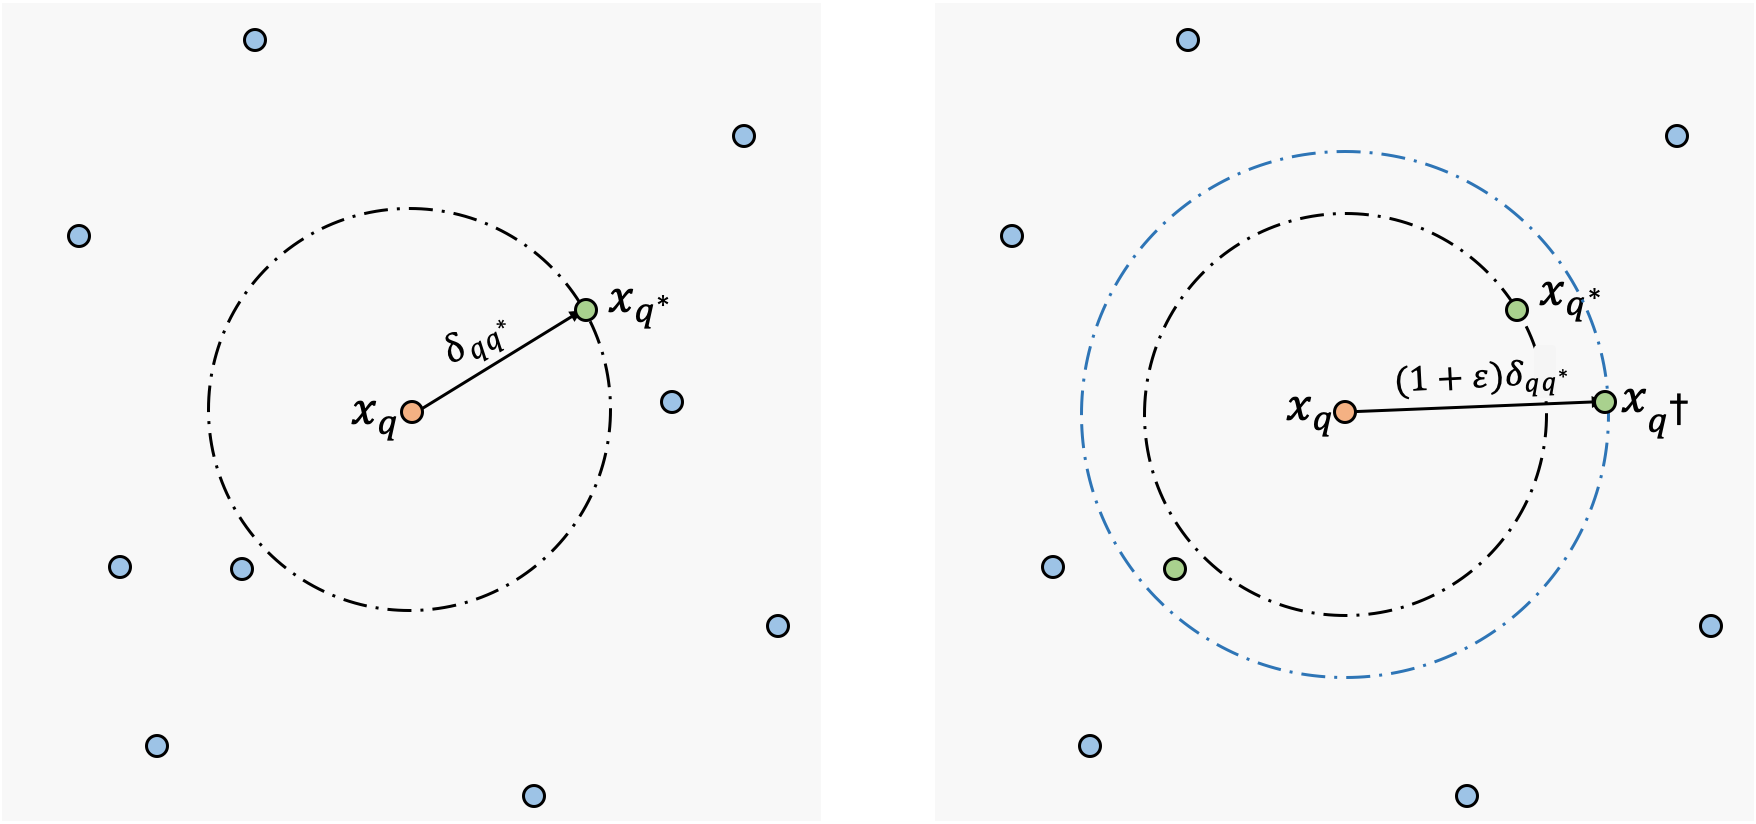
\includegraphics[width=0.8\linewidth]{/Users/fche0019/git/mlann_github/paper/figures/ann} 

}

\caption{Illustration of approximate nearest neighbors (right) compared to exact nearest neighbors (left). The left subplot shows the distance from the true nearest neighbor point $x_{q^*}$ to the query point $x_q$ is $\delta_{q{q^*}}$, while the right subplot shows that the $(1+\varepsilon)$ -approximate nearest neighbors (green points) lie within $(1+\varepsilon) \delta_{q{q^*}}$ radius from $x_q$. }\label{fig:ann}
\end{figure}

\protect\hyperlink{ref-Aumuller2020-nk}{Aumüller, Bernhardsson, and Faithfull} (\protect\hyperlink{ref-Aumuller2020-nk}{2020}) developed a benchmark tool\footnote{available at \url{http://ann-benchmarks.com/}.} and evaluated a number of contemporary approximate nearest neighbor searching methods. Among these methods, Annoy and HNSW are the most competitive ones, therefore, we consider these algorithms in our study. Furthermore, since Annoy is a tree-based method and HNSW is a graph-based method, there is one algorithm from each large class of ANN algorithms. Finally, we will also use k-d trees since this is one of the most widely used algorithms for (approximate) nearest neighbor search. In addition, k-d trees also allow for the special case of exact nearest neighbor search through appropriate selection of the tuning parameters, thus easily allowing us to isolate the effect of using approximate nearest neighbors in manifold learning algorithms. We now briefly describe the approximate nearest neighbor algorithms used in our evaluation, namely, k-d trees, Annoy, and HNSW.

\hypertarget{k-d-trees}{%
\subsubsection*{k-d trees}\label{k-d-trees}}
\addcontentsline{toc}{subsubsection}{k-d trees}

The k-d tree (\protect\hyperlink{ref-Bentley1975-zo}{Bentley 1975}), is a binary tree structure that can be exploited for nearest neighbor search. Each node is associated with a partition of \(p\)-dimensional space \(\mathcal{P}_g\) (hereafter the node and partition will be treated interchangeably). A node has two children --- a left child node and a right child node --- formed by splitting \(\mathcal{P}_g\) by an axis-orthogonal hyper-plane. By a variant of k-d trees proposed by \protect\hyperlink{ref-Friedman1977-dh}{Friedman, Bentley, and Finkel} (\protect\hyperlink{ref-Friedman1977-dh}{1977}), the splitting dimension \(l_g^*\) for the splitting hyperplane is chosen to maximize spread. The splitting value \(c_g^*\) is chosen as the median along the splitting dimension of all points in \(\mathcal{P}_g\). The process of building a k-d tree is shown in Algorithm \ref{alg:buildkdtree}. Note that while Algorithm \ref{alg:buildkdtree} will construct a tree with terminal nodes that include no more than one data point, variants of k-d trees allow for multiple points in the terminal nodes.

Once a k-d tree is constructed, nearest neighbors can be searched in time proportional to \(O(\log(N))\). Nearest neighbor search begins at the root node and determines whether the query point belongs to the partition of the left child node or right child node. The search moves to the child node to which it belongs and this process is iterated until a terminal node \(\mathcal{P}_T\) is reached. The distance from the query point to \(x_i\in\mathcal{P}_T\) is set to the current shortest distance \(\delta^*\) and \(x_i\) to the current nearest neighbor. The search algorithm then unwinds back through the tree. At each parent node, there will be one sibling node that has been searched and one sibling node yet to be searched. Denote the latter as \(\mathcal{P}_{g^*}\). The tightest bounding box containing all \(x_i:x_i\in\mathcal{P}_{g^*}\) is computed as well as a hyper-sphere of radius \(\delta^*\) around the query point. If the hyper-sphere and bounding box do not intersect, then the nearest neighbor cannot lie in \(\mathcal{P}_{g^*}\) and the branch starting from this node can be disregarded. Otherwise, this branch must also be searched. Pseudocode for a recursive procedure used to find the nearest neighbor \(x_{q^*}\) of a query point \(x_q\) is given in Algorithm \ref{alg:searchkdtree}. This search is initialized by evaluating this procedure at the root node and initializing the current closest distance at \(\delta^*=\infty\).

The algorithm as described above will find exact nearest neighbors with \(O(\log(N))\) operations on average. However, if approximate rather than exact nearest neighbors are desired, further speed up can be achieved by setting the radius of the hypersphere at Line 11 and Line 18 of Algorithm \ref{alg:searchkdtree} to \(\delta^*/(1+\varepsilon)\). This increases the number of branches of the tree eliminated from the search. In subsequent sections, we tune \(\varepsilon\) to trade off between speed and accuracy. In all cases below where exact nearest neighbors are computed, we employ k-d trees with \(\varepsilon=0\). We also note that while Algorithm \ref{alg:searchkdtree} finds the nearest neighbor, it can be generalized to finding \(K\) nearest neighbors by replacing the current smallest distance and current closest node with the current \(K\)-th smallest distance and current \(K\)-th closest node respectively.

\hypertarget{annoy}{%
\subsubsection*{Annoy}\label{annoy}}
\addcontentsline{toc}{subsubsection}{Annoy}

Annoy {[}Approximate Nearest Neighbors Oh Yeah; \protect\hyperlink{ref-Bernhardsson2016-tf}{Spotify} (\protect\hyperlink{ref-Bernhardsson2016-tf}{2016}){]} is a C++ library with Python bindings that implements an alternative tree-base algorithm for nearest neighbor search. While sharing some similarities, Annoy differs from k-d trees in two main ways. First, rather than using a single tree, the Annoy algorithm constructs a forest of randomly constructed trees that can be searched in parallel. Second, while Annoy builds trees by constructing splitting hyperplanes, unlike k-d trees, these hyperplanes are not axis-orthogonal. Instead, for each split, Annoy chooses two points at random and sets the splitting hyperplane to be equidistant from these two points. Each node (including terminal nodes) is associated with a partition containing multiple (at most \(\kappa\)) points. One such tree is shown in Figure \ref{fig:annoy}.



\begin{figure}

{\centering 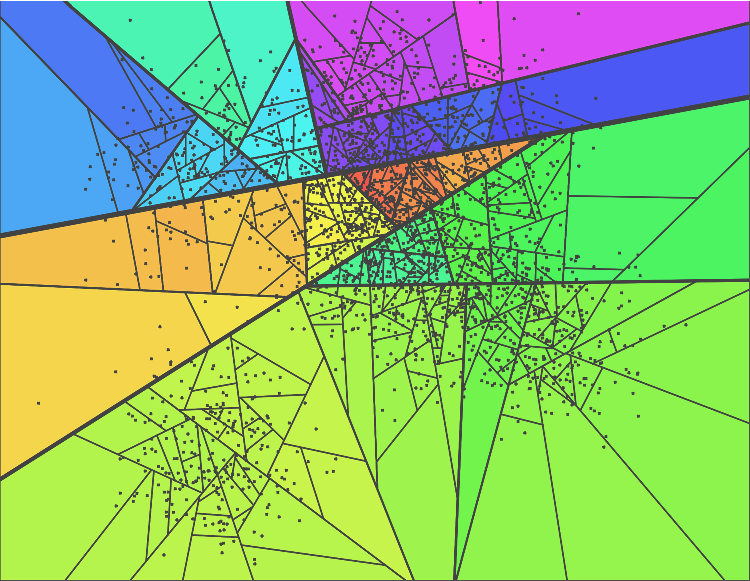
\includegraphics[width=.49\linewidth]{/Users/fche0019/git/mlann_github/paper/figures/annoy1} 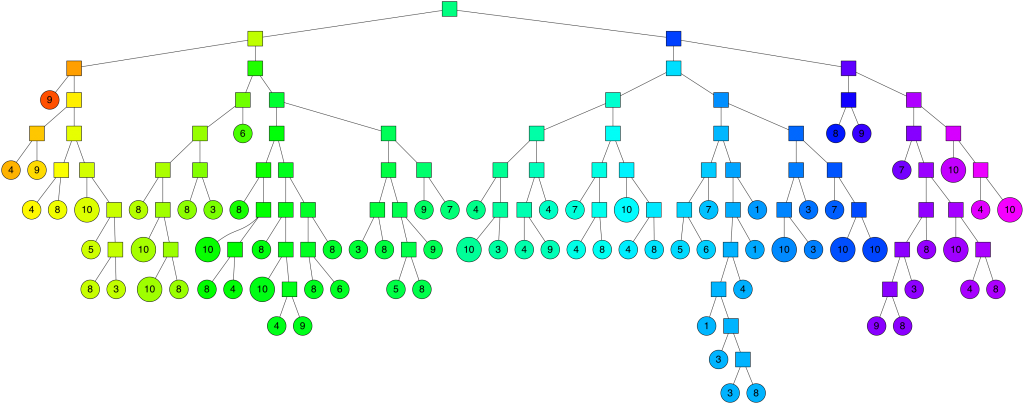
\includegraphics[width=.49\linewidth]{/Users/fche0019/git/mlann_github/paper/figures/annoy2} 

}

\caption{The splitting process of Annoy (on the left) and the corresponding binary tree (on the right) reproduced from \protect\hyperlink{ref-Bernhardsson2015-slides}{Bernhardsson} (\protect\hyperlink{ref-Bernhardsson2015-slides}{2015}).}\label{fig:annoy}
\end{figure}

Annoy searches for nearest neighbors on all trees in the forest in parallel. The search for nearest neighbor candidates on a single tree does share some similarities with nearest neighbor search on k-d trees. In particular, the search begins from the root node and iteratively moves to the child node associated with a partition containing the query point. Once a terminal node is reached, points within this node are considered as nearest neighbor candidates. However, Annoy does not unwind each tree in the same fashion as k-d trees. Instead, Annoy maintains a priority queue (shared across all trees of the forest) of the splitting hyperplanes closest to the query point. If the distance from the query point to a splitting hyperplane is less than some threshold \(\eta\), then the opposite side of the hyperplane is also searched. Increasing the threshold throughout allows more points to be considered as nearest neighbor candidates.

Once the union of candidate points across all trees contains \textit{search\_k} points, searching the forest ends. Distances are computed to each point in the candidate sets and approximate nearest neighbors found. The accuracy-performance trade-off is controlled by two parameters, the number of trees, \textit{n\_trees}, and the size of the candidate set, \textit{search\_k}. In both cases, larger values will improve the accuracy of nearest neighbor search at the cost of slower performance. Choosing a larger value of \textit{n\_trees} also increases the demand for storage. A full description of the Annoy is provided in Algorithm \ref{alg:annoypre} and \ref{alg:annoyquery}.

\hypertarget{hierarchical-navigable-small-world-graphs-hnsw}{%
\subsubsection*{Hierarchical Navigable Small World graphs (HNSW)}\label{hierarchical-navigable-small-world-graphs-hnsw}}
\addcontentsline{toc}{subsubsection}{Hierarchical Navigable Small World graphs (HNSW)}

Hierarchical Navigable Small World (\protect\hyperlink{ref-Malkov2020-jp}{Malkov and Yashunin 2020}) is a graph-based approximate nearest neighbor searching method. Before providing an overview of HNSW, it is instructive to describe how a graph can be greedily traversed to search for the approximate nearest neighbor of a query point. This will be done using Figure \ref{fig:naive} as an example where each node of the graph corresponds to a data point and the query point is colored red. Throughout we assume that the edges of the graph connect points that are (approximately) close to one another and searching proceeds via the principle that a \emph{neighbor's neighbor is likely to be a neighbor}. First, a random entry point is selected (suppose this is J). The distance between the query point and entry point is computed and the current nearest point is set to the entry point. Next, the distances between the query point and the current nearest point's neighbors (G, I, and K) are computed. If at least one neighboring point is closer to the query point than the current nearest point, then the current nearest point is updated. In Figure \ref{fig:naive} this will be K. The algorithm continues and terminates when there are no unvisited neighboring points that are closer to the query point than the current nearest point. In Figure \ref{fig:naive} this will be at point L. A general description of this greedy search is provided in Algorithm \ref{alg:hnsw}.

\begin{figure}

{\centering 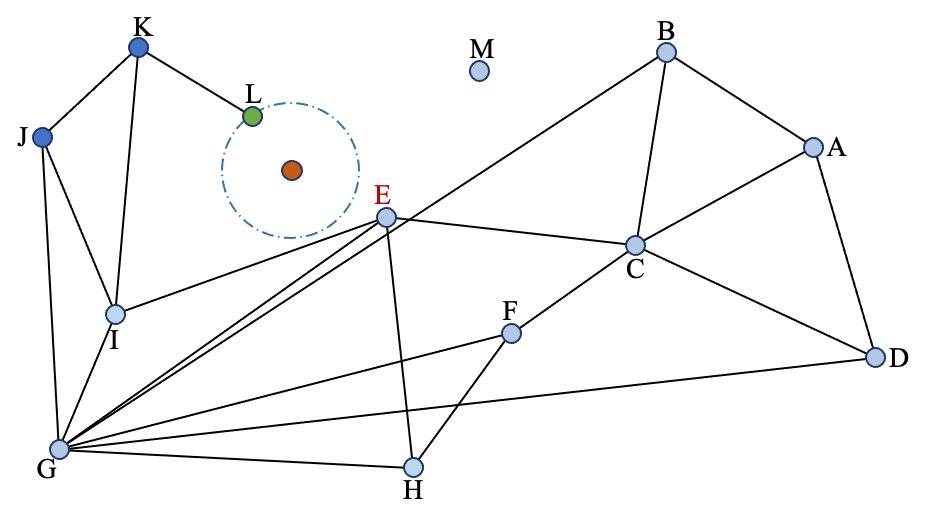
\includegraphics[width=0.6\linewidth]{/Users/fche0019/git/mlann_github/paper/figures/naive_search} 

}

\caption{An example of naive nearest neighbor searching in HNSW. For the red query point, the approximate nearest neighbor is L if the entry point is J. For entry point E or M, the greedy search would fail at approximate nearest neighbor E since the true nearest neighbor is L. }\label{fig:naive}
\end{figure}

This greedy search does have some shortcomings, in particular, it will fail for some entry points (for instance E or M in Figure \ref{fig:naive}) and can be slow when the number of data points is large. To overcome the second issue, HNSW constructs a hierarchy of graphs, with each increasing layer involving fewer and fewer points. This is depicted in Figure \ref{fig:hnsw}. Greedy search on the more sparse levels of the hierarchy acts as an expressway mechanism to quickly reach a region of space where nearest neighbors are likely to be found. In Figure \ref{fig:hnsw}, the algorithm begins at the randomly chosen red point on Layer 2 (\(x_e\)) and by greedy search reaches the blue point on Layer 2 (\(x_b\)). This point becomes the entry point for a greedy search on Layer 1 of the graph. This process is iterated until an approximate nearest neighbor is found on the dense graph at Layer 0 (the green point \(x_a\) in Figure \ref{fig:hnsw}).

The only issue remaining is the construction of the graphs at each level of the hierarchy. This process follows a similar idea to approximate nearest neighbor search of a query point only with each data point sequentially inserted into the graph as a query point. Once approximate nearest neighbors are found for a data point, \textit{n\_links} edges are added to the graph between the data point and its approximate nearest neighbors, where \textit{n\_links} can be chosen to trade off between speed and accuracy. A maximum layer \(L^*\) is randomly chosen for each point such that the point is only inserted into graphs corresponding to Layer \(L^*\) and below. Generating \(L^*\) from a distribution with exponentially decaying tails ensures that the high layers are sparse. Some pruning of unnecessary edges in each graph is also recommended with details provided in \protect\hyperlink{ref-Malkov2020-jp}{Malkov and Yashunin} (\protect\hyperlink{ref-Malkov2020-jp}{2020}).



\begin{figure}

{\centering 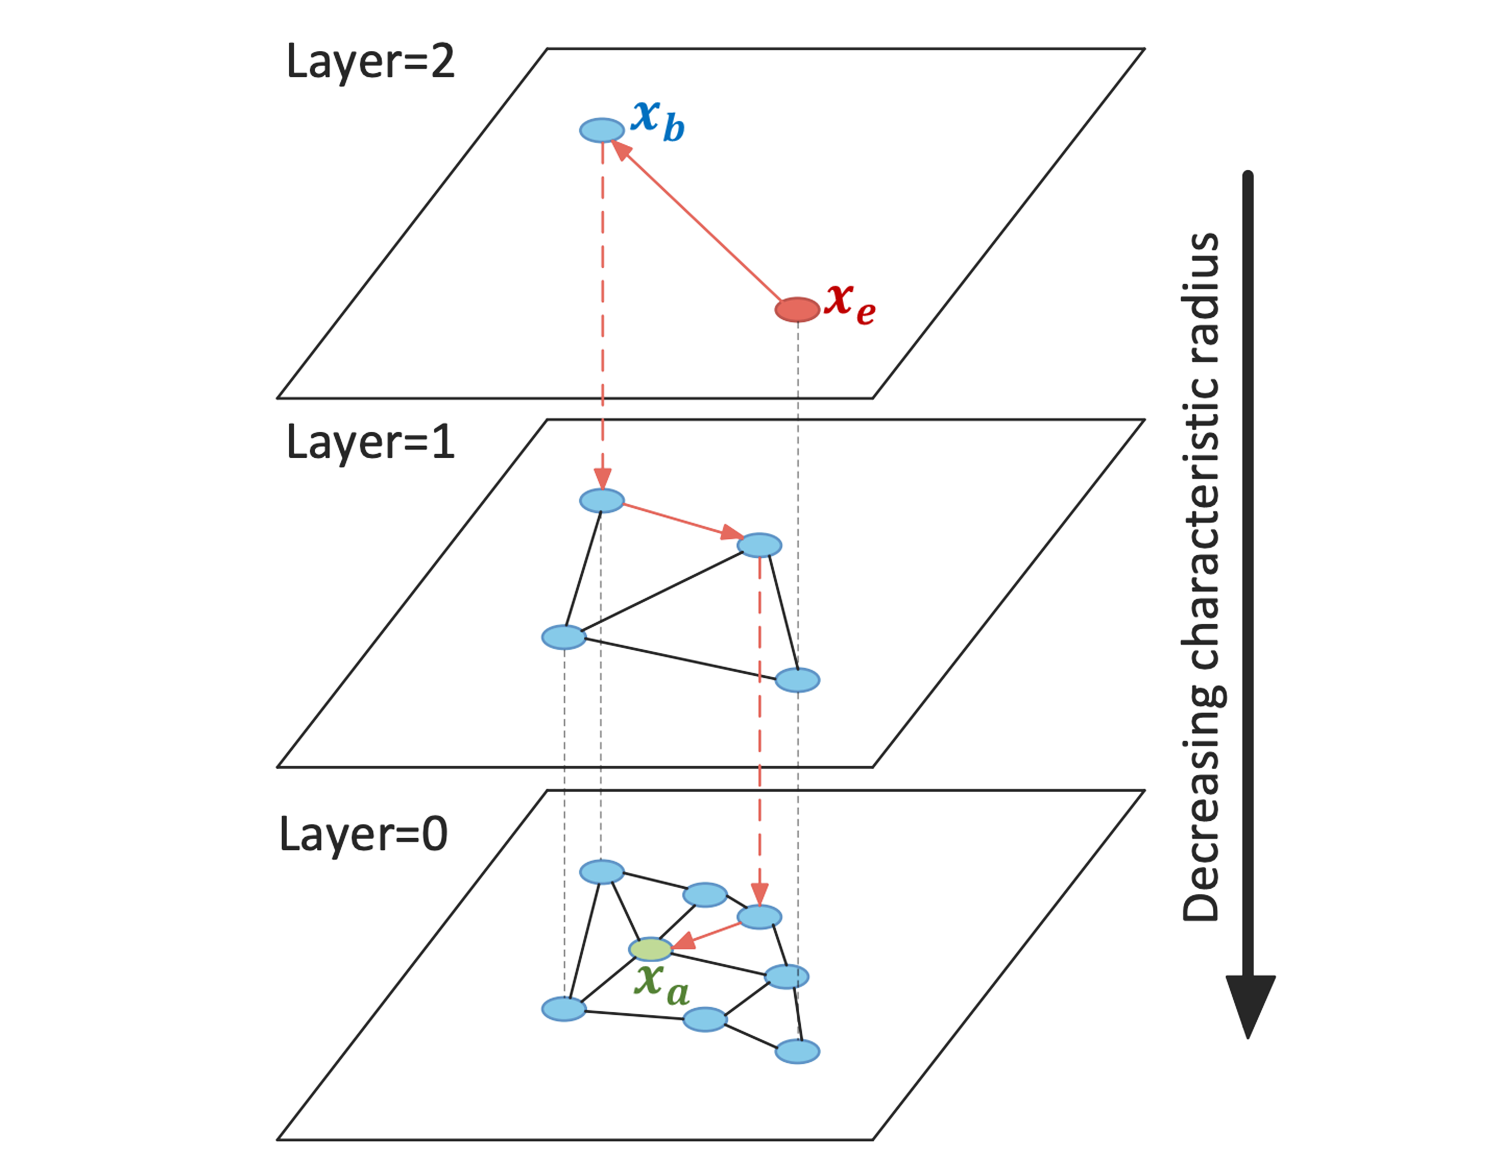
\includegraphics[width=0.6\linewidth]{/Users/fche0019/git/mlann_github/paper/figures/hnsw} 

}

\caption{The hierarchical structure built from HNSW reproduced from \protect\hyperlink{ref-Malkov2020-jp}{Malkov and Yashunin} (\protect\hyperlink{ref-Malkov2020-jp}{2020}). The red entry point \(x_e\) is randomly chosen on the top layer. The greedy search follows the red arrow until an approximate nearest neighbor \(x_a\) is found (shown green).}\label{fig:hnsw}
\end{figure}

\hypertarget{qualitymeasure}{%
\subsection{Quality measures for manifold learning embedding}\label{qualitymeasure}}

To examine the effect of using approximate nearest neighbor algorithms in manifold learning, measures of the quality of a low dimensional representation must be defined. There are a number of criteria that we consider, all of which measure the extent to which the nearest neighbor structure of the output points resembles the nearest neighbor structure of the input points. That is, all criteria measure the extent to which the topology of the manifold is preserved while the final criterion we consider (the Procrustes measure), additionally measures the extent to which the local geometry is preserved. For ease of comparison, we adjust all quality measures so that higher values of a measure indicate a higher quality embedding.

Recall that \(U_K(i)\) was defined as the set of points \(j\) such that \(x_j\) is one of the \(K\)-nearest neighbors of \(x_i\). We now also define \(V_K(i)\) as the nearest neighborhood of observation \(i\) in the output space, i.e.~a set of points \(j\) such that \(y_j\) is one of the \(K\)-nearest neighbors of \(y_i\). We define the neighborhood ranking of \(x_j\) with respect to \(x_i\) as \(\rho_{ij} =|\{\ell: \delta_{i \ell}<\delta_{i j}\} |\). For example, if \(x_j\) is the nearest neighbor of \(x_i\), then \(\rho_{ij}=1\) since only \(\delta_{ii}<\delta_{ij}\), where we assume without loss of generality that all input points are distinct. In case of tied distances, \(\rho_{ij} =\left|\big\{\ell: \delta_{i \ell}<\delta_{i j} \text { or }(\delta_{i \ell}=\delta_{i j} \text { and } \ell<j)\big\}\right|\). The neighborhood rankings of output points, denoted \(r_{ij}\), are similarly defined using \(d_{ij}\) in place of \(\delta_{ij}\). The value of \(K\) used to compute quality measures need not be the same as that used in the manifold learning algorithms, however, in all our simulations, we also set \(K=20\) for the purpose of computing quality measures.

\hypertarget{local-continuity-meta-criterion-lcmc}{%
\subsubsection*{Local Continuity Meta-Criterion (LCMC)}\label{local-continuity-meta-criterion-lcmc}}
\addcontentsline{toc}{subsubsection}{Local Continuity Meta-Criterion (LCMC)}

\protect\hyperlink{ref-Chen2009-su}{Chen and Buja} (\protect\hyperlink{ref-Chen2009-su}{2009}) proposed the local continuity criterion (LCMC) defined as
\begin{equation}\label{eq:LCMC}
  \text{LCMC}(K)=\frac{1}{N K} \sum_{i=1}^{N}\Big(\big| U_K(i) \bigcap V_K(i) \big| - \frac{K^{2}}{N-1}\Big).
\end{equation}
The LCMC computes the average size of the overlap between the \(K\)-nearest neighborhood in the output space and \(K\)-nearest neighborhood in the input space. The value of LCMC\((K)\), is bounded between zero and one with values closer to one indicating a larger overlap between nearest neighborhoods and therefore better quality embedding.

\hypertarget{trustworthiness-continuity-tc}{%
\subsubsection*{Trustworthiness \& Continuity (T\&C)}\label{trustworthiness-continuity-tc}}
\addcontentsline{toc}{subsubsection}{Trustworthiness \& Continuity (T\&C)}

\protect\hyperlink{ref-Venna2006-nd}{Venna and Kaski} (\protect\hyperlink{ref-Venna2006-nd}{2006}) defined two quality measures, trustworthiness and continuity, that respectively distinguish two type of errors. For the first type of error, \(y_j\) is among the \(K\) nearest neighbors of \(y_i\) (i.e.~observations close in output space) but \(x_j\) is not among the \(K\)-nearest neighbors of \(x_i\) (i.e.~observations not close in the input space). Using all such points for each \(i\), the trustworthiness of the embedding can be calculated as
\begin{equation}\label{eq:trustworthiness}
  M_{T}(K)=1-\frac{2}{G_{K}} \sum_{i=1}^{N} \sum\limits_{\begin{subarray}{c}j \in V_{K}(i)\\j \notin U_{K}(i)\end{subarray}}(\rho_{ij}-K),
\end{equation}
where the normalizing factor
\[
  G_{K}=\left\{
    \begin{array}{ll}
      N K(2 N-3 K-1) & \text { if } K<N / 2, \\
      N(N-K)(N-K-1) & \text { if } K \geq N / 2.
    \end{array}
  \right.
\]

This is bounded between zero and one, with values closer to one indicating a higher-quality representation. In contrast to LCMC, Trustworthiness uses information on the rankings of interpoint distances. In particular, points that are incorrectly included as nearest neighbors in the output space are penalized more when they are further away in the input space (\(\rho_{ij}\) is high).

For the second type of error, \(x_j\) is among the \(K\) nearest neighbors of \(x_i\) (i.e.~observations close in input space) but \(y_j\) is not among the \(K\)-nearest neighbors of \(y_i\) (i.e.~observations not close in the output space). Using these points, the continuity is defined as
\begin{equation}\label{eq:continuity}
  M_{C}(K)=1-\frac{2}{G_{K}} \sum_{i=1}^{N} \sum_{\begin{subarray}{\ell}j \in U_{K}(i) \\j\notin V_{K}(i)\end{subarray}}(r_{ij}-K).
\end{equation}
This is also normalized between zero and one and higher values indicate a higher-quality representation. Errors made for points further away in the output space (\(r_{ij}\)) are penalized to a greater extent.

\hypertarget{mean-relative-rank-errors-mrres}{%
\subsubsection*{Mean Relative Rank Errors (MRREs)}\label{mean-relative-rank-errors-mrres}}
\addcontentsline{toc}{subsubsection}{Mean Relative Rank Errors (MRREs)}

\protect\hyperlink{ref-Lee2008-dy}{J. Lee and Verleysen} (\protect\hyperlink{ref-Lee2008-dy}{2008}) developed two measures known as mean relative rank errors, based on similar principles as Trustworthiness and Continuity. These are defined as
\begin{equation}\label{eq:MRREs}
\begin{aligned}
  & W_{n}(K)=\frac{1}{H_{K}} \sum_{i=1}^{N} \sum_{j \in U_{K}(i)} \frac{|\rho_{ij}-r_{ij}|}{\rho_{ij}}, \\
  & W_{\nu}(K)=\frac{1}{H_{k}} \sum_{i=1}^{n} \sum_{j \in V_{k}(i)} \frac{|\rho_{ij}-r_{ij}|}{r_{ij}},
\end{aligned}
\end{equation}
where \(H_K\) is the normalizing factor defined as
\[
  H_{K}=n \sum_{i=1}^{K} \frac{|N-2 i+1|}{i}.
\]

The set of observations \(j\) that lie in the \(K\)-nearest neighborhood of \(i\) in both the input and output space do not affect the Trustworthiness and Continuity measures. In contrast, Mean Relative Rank Errors will penalize such points, particularly when the ranking of the distance between \(x_i\) and \(x_j\) differs substantially from the ranking of the distance between \(y_i\) and \(y_j\). For ease of comparison to other quality measures, we will report \(1-W_{n}(K)\) and \(1-W_{\nu}(K)\) so that larger values indicate a better quality embedding.

\hypertarget{co-ranking-matrix-q_nxk}{%
\subsubsection*{\texorpdfstring{Co-ranking Matrix (\(Q_{NX}(K)\))}{Co-ranking Matrix (Q\_\{NX\}(K))}}\label{co-ranking-matrix-q_nxk}}
\addcontentsline{toc}{subsubsection}{Co-ranking Matrix (\(Q_{NX}(K)\))}

The co-ranking matrix criterion is defined as
\begin{equation}\label{eq:Q_NX}
  Q_{NX}(K)=\frac{1}{K N} \sum_{k=1}^{K} \sum_{\ell=1}^{K} q_{k\ell},
\end{equation}
where \(q_{k\ell}\) is the element in row \(k\) and column \(\ell\) of the co-ranking matrix defined as
\begin{equation}\label{eq:coRanking}
  q_{k\ell}=|\{(i, j): \rho_{i j}=k \text { and } r_{i j}=\ell\}|.
\end{equation}
For instance, the element in the first row and column of \(Q\), \(q_{11}\), denotes the number of pairs of observations for which the second observation is the nearest neighbor of the first observation in both the input and output space. The range of the criterion is \(Q_{N X}(K) \in[0,1]\), where 1 indicates a more accurate representation. It is also worth noting that the T\&C, MRREs, and LCMC can be expressed in terms of the co-ranking matrix with details provided by \protect\hyperlink{ref-Lee2008-dy}{J. Lee and Verleysen} (\protect\hyperlink{ref-Lee2008-dy}{2008}).

\hypertarget{procrustes-measure-rxy}{%
\subsubsection*{\texorpdfstring{Procrustes measure (\(R(X,Y)\))}{Procrustes measure (R(X,Y))}}\label{procrustes-measure-rxy}}
\addcontentsline{toc}{subsubsection}{Procrustes measure (\(R(X,Y)\))}

As a final criterion for measuring the quality of a low-dimensional representation, we consider the Procrustes measure (\protect\hyperlink{ref-Goldberg2009-tb}{Goldberg and Ritov 2009}). The idea rests on the definition of a manifold as a being locally isomorphic to Euclidean space. More concretely, the Procrustes measure considers observations in the neighborhood of \(x_i\), i.e observations \(x_j:j\in U_K(i)\). The Procrustes rotation finds a \(d\times p\) matrix \(A\) and a \(d\)-vector \(b\) that projects \(x_j\) onto a \(d\)-dimensional subspace. The aim is for the projected (and translated) points \(Ax_j+b\) to be close to the corresponding output points \(y_j\) for \(j\in U_K(i)\). This measure of closeness is the Procrustes statistic which for observation \(i\), is defined as
\begin{equation}\label{eq:procstats}
  G_i= \inf _{\{A,b: A^{\prime} A=I\}} \sum_{j\in U_K(i)}\|x_{j}-A y_{j}-b\|^{2}.
\end{equation}
An overall measure of quality is found given by
\begin{equation}\label{eq:procmeasure}
  G=\frac{1}{n}\sum\limits_{i=1}^N\frac{G_i}{\sum_{j\in U_K(i)}\|x_{j}\|^{2}}\,
\end{equation}
where the denominator is a normalizing factor that ensures \(G\) will lie between zero and one. An advantage of this measure is that it will favor embeddings that preserve the geometric properties (e.g.~distances, angles) of the manifold. Since larger values of \(G\) indicate a worse representation, to ease comparison with other measures we report \(1-G\).

\hypertarget{experiment}{%
\section{Experiments}\label{experiment}}

\hypertarget{mnist-dataset}{%
\subsection{MNIST dataset}\label{mnist-dataset}}

The MNIST database {[}Modified National Institute of Standards and Technology database; \protect\hyperlink{ref-lecun2010mnist}{LeCun, Cortes, and Burges} (\protect\hyperlink{ref-lecun2010mnist}{2010}){]} is a commonly used benchmark dataset for dimension reduction techniques, consisting of 60,000 grayscale images of handwritten digits in a training set, and 10,000 grayscale images in a test set. It was constructed from a larger database called NIST. In the original NIST dataset, images in the training data were hand-written by American Census Bureau employees (Special Database 3, SD-3), while images in the test data were handwritten by high school students (Special Database 1, SD-1). \protect\hyperlink{ref-lecun2010mnist}{LeCun, Cortes, and Burges} (\protect\hyperlink{ref-lecun2010mnist}{2010}) normalized the size of the NIST images and centered them in a \(28\times 28=784\) pixel field. Then they mixed the samples from both SD-3 and SD-1 to form the MNIST dataset, where the training set contains 30,000 images from SD-3 and 30,000 images from SD-1, while the test set is composed of 5,000 images from SD-3 and 5,000 images from SD-1.

To examine manifold learning using ANN techniques, we use the MNIST test set of \(N=10,000\) observations, with a dimension equal to the number of pixels (\(p=784\)). The embedding dimension for manifold learning is set as \(d=5\). We apply different combinations of manifold learning algorithms and ANN methods to the data, recording the computational time and calculating the embedding quality measures discussed in Section \ref{qualitymeasure}. All experiments were run in parallel on a high performance computing cluster with 2.70GHz Xeon-Gold-6150 CPUs.

\hypertarget{mnistresults}{%
\subsection{Experimental results}\label{mnistresults}}

Choosing different values of the tuning parameters for approximate nearest neighbor algorithms allows for a trade-off between computational time and accuracy. For k-d trees, we consider values of \(\varepsilon\) ranging from 0 to 5 in increments of 0.1. Note that setting \(\varepsilon=0\) allows us to compute exact nearest neighbors. For Annoy, we set values of \textit{n\_trees} ranging from 2 to 100 in increments of 2 and fix \textit{search\_k} as 500. For HNSW, we set \textit{n\_links} to range from 2 to 200 incremented by 2. For each set of parameter values, we record the computational time taken to find the nearest neighbor graph. We also record the recall rate defined as the proportion of observations correctly classified as nearest neighbors.

These results are summarized in Figure \ref{fig:recall}, where each point represents the recall and computational time for an ANN algorithm with a specific set of tuning parameters.
A vertical line indicating the exact nearest neighbors is also added to the plot as a baseline for the ANN methods with a similar line added to subsequent figures that compare the accuracy and computation time. As expected, each ANN method shows a trade-off between computational time and accuracy with lower computational time associated with lower recall rates. If a curve lies entirely to the top and left of another curve, this suggests that one ANN method dominates the other with respect to the recall rate. Figure \ref{fig:recall} shows that the best performing ANN method is Annoy, followed by HNSW followed by k-d trees. This is in line with the finding of \protect\hyperlink{ref-Aumuller2020-nk}{Aumüller, Bernhardsson, and Faithfull} (\protect\hyperlink{ref-Aumuller2020-nk}{2020}) who show that Annoy and HNSW both outperform k-d trees.

While the experiment gives a clear ranking of ANN methods according to recall rate, this ranking may not hold when the ANN methods are used as the first step of a manifold learning algorithm, and accuracy is defined according to quality measures of the resulting embedding. For the remainder of this section, we construct similar plots to Figure \ref{fig:recall}, but with measures of the quality of a manifold learning embedding rather than recall rate.

\begin{figure}

{\centering 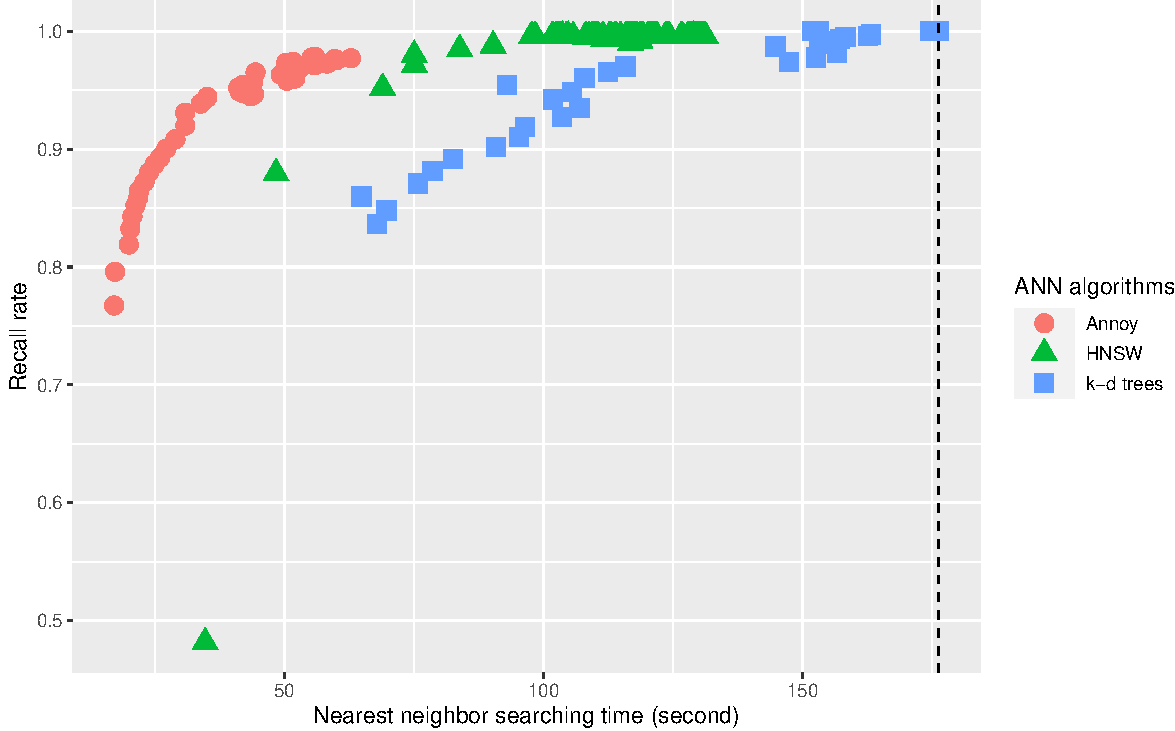
\includegraphics[width=0.8\linewidth]{mlann_jcgs_files/figure-latex/recall-1} 

}

\caption{The comparison plot of recall rate for three ANN methods, k-d trees, Annoy, and HNSW. The points show the change of computation time (second) against the ANN recall rate for different sets of parameter values. Points that are higher in recall rate and less in computation time (to the left) are relatively better. The black vertical line indicates the computation time for finding exact nearest neighbors. }\label{fig:recall}
\end{figure}

\begin{figure}

{\centering 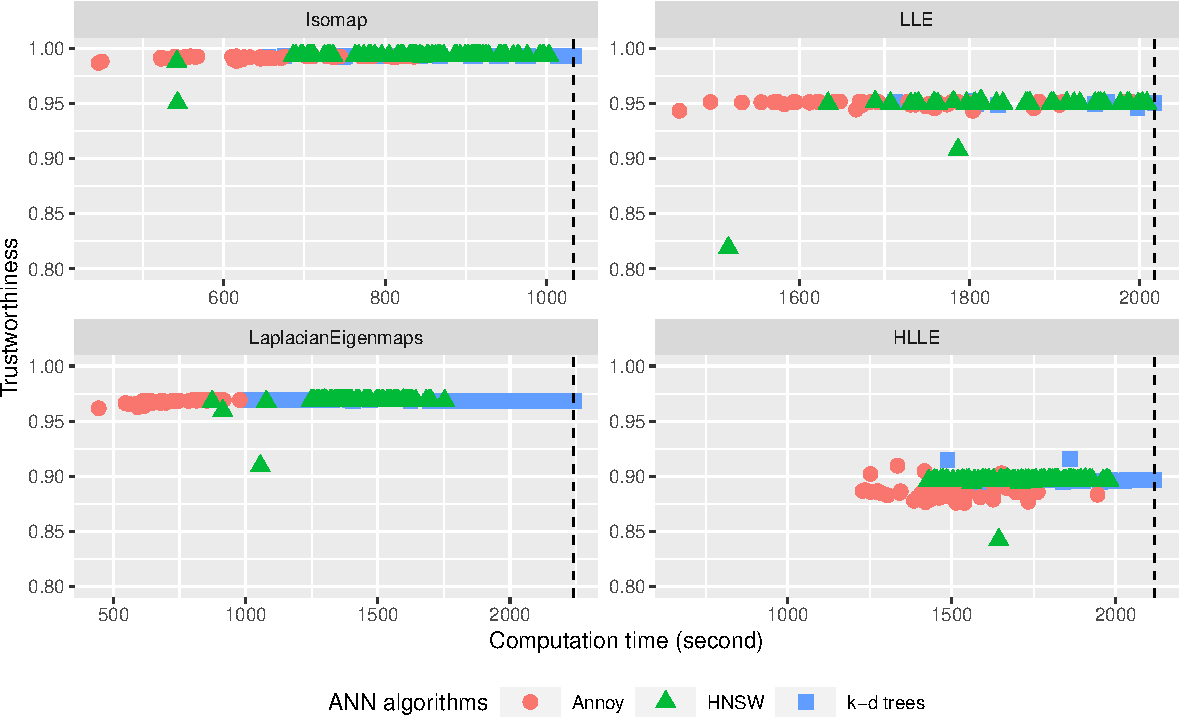
\includegraphics[width=1\linewidth]{mlann_jcgs_files/figure-latex/iso-1} 

}

\caption{Trustworthiness against computation time for Annoy, HNSW and k-d trees with different parameter values in four manifold learning methods. Top-left: Isomap; Top-right: LLE; Bottom-left: Laplacian Eigenmaps, Bottom-right: Hessian LLE. Points that are higher in Trustworthiness and less in computation time (to the left) are relatively better. }\label{fig:iso}
\end{figure}

Figure \ref{fig:iso} shows the performance of different combinations of ANN and manifold learning algorithms according to the Trustworthiness measure. Once again ANN methods with a curve closer to the top left of the plot are to be preferred. Each panel refers to a different manifold learning algorithm method, namely Isomap (top-left), LLE (top-right), Laplacian Eigenmaps (bottom-left), and Hessian LLE (bottom-right). Figure \ref{fig:iso} provides a number of insights. First, the use of approximate nearest neighbors can reduce the computational time taken to carry out manifold learning. For example, using k-d trees with Isomap allows computational time to be reduced from around 1,030 seconds to 650 seconds. This reduction in computational time is greatest when Annoy is used, a result consistent with Figure \ref{fig:recall}. The speed-up is also particularly noticeable for Laplacian Eigenmaps where Annoy can achieve a roughly four-fold improvement in computational time compared to exact nearest neighbors. This result can be explained by the fact that finding the nearest neighbors graph represents more of a computational bottleneck for Laplacian Eigenmaps compared to other algorithms. Second, in a result that stands in contrast to Figure \ref{fig:recall}, the improvement in computational time does not come at the cost of substantially lower Trustworthiness. In fact, the effect of using a different manifold learning algorithm seems to have a much greater impact on Trustworthiness than the use of an approximate nearest neighbor algorithm. For example, the Trustworthiness is almost always between 0.98 and 1 when Isomap is used (the best performing algorithm for this particular dataset), while it is almost always between 0.87 to 0.92 for Hessian LLE (the worst-performing algorithm for this particular dataset). As a minor caveat to the conclusion that ANN has a negligible impact on embedding accuracy, we note that HNSW has a small number of very inaccurate embeddings that lead to a substantially lower Trustworthiness. This may be explained by the propensity of the greedy search upon which HNSW is built to return nearest neighbors that are quite far from the true nearest neighbor.

\begin{figure}

{\centering 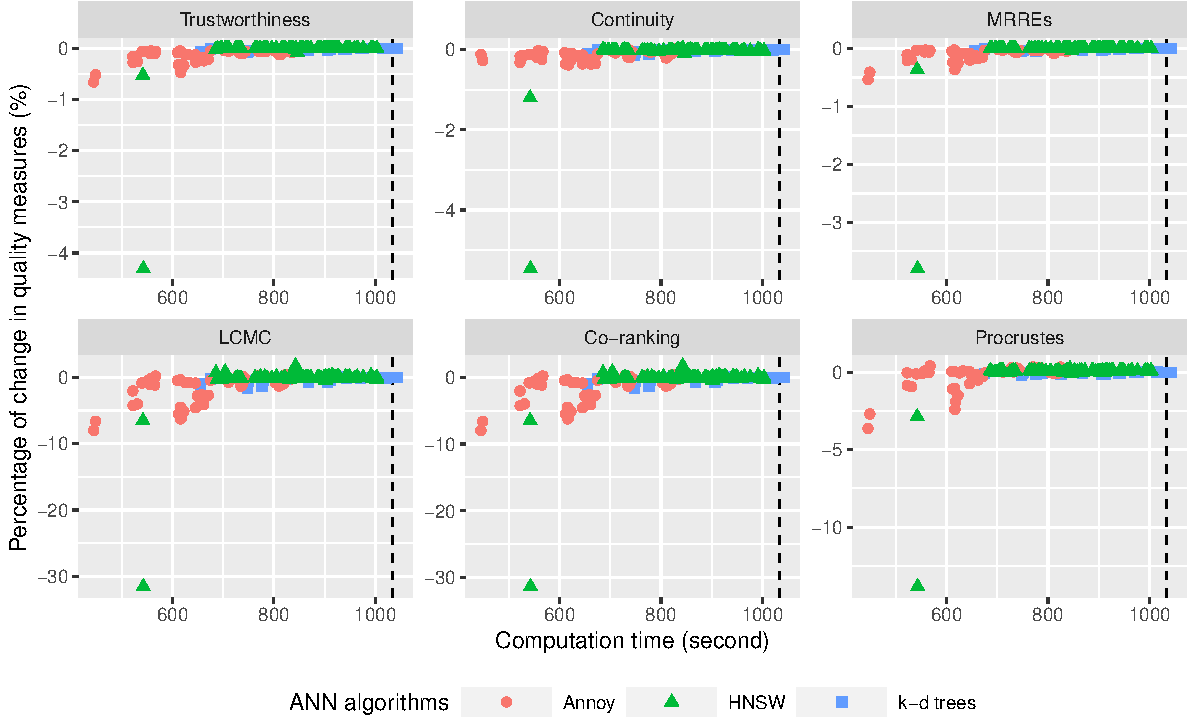
\includegraphics[width=1\linewidth]{mlann_jcgs_files/figure-latex/iso6measure-1} 

}

\caption{Comparison of Isomap embedding quality measures against computation time for three ANN methods, Annoy, HNSW, and k-d trees. The percentage change compared to true nearest neighbors of six quality measures are shown in the order of Trustworthiness, Continuity, MRREs, LCMC, Co-ranking matrix, and Procrustes measure. }\label{fig:iso6measure}
\end{figure}

The results from Figure \ref{fig:iso} are, for the most part, robust to the use of metric used to evaluate embedding quality. For instance, Figure \ref{fig:iso6measure} shows results of percentage change for all quality measures discussed in Section \ref{qualitymeasure} for Isomap. For all measures, the computational time of the algorithm can be cut in half with an associated reduction in the accuracy of less than 10\% (with a few exceptions due to the instability of HNSW). Similar conclusions can be drawn for LLE and Laplacian Eigenmaps so these figures\footnote{available at \url{https://github.com/ffancheng/paper-mlann/tree/public/paper/figures/public}.} are omitted for brevity.
On the other hand, Figure \ref{fig:hllemeasure} does show that for Hessian LLE, HNSW can achieve a higher level of accuracy for some measures (Continuity, LCMC, Co-ranking, and Procrustes), even compared to exact nearest neighbors. While this result is quite counter-intuitive, it should be noted that Hessian LLE performs considerably worse than Isomap (in general Isomap achieves an LCMC of above 0.3 for Isomap, the corresponding figure never exceeds 0.2 for Hessian LLE).
This can also be inferred from Table \ref{tab:nnmeasure} where six embedding quality measures using the exact nearest neighbors are shown for four different manifold learning algorithms. In general, Isomap outperforms the other three methods while Hessian LLE performs the worst in terms of all six quality measures.

\begin{figure}

{\centering 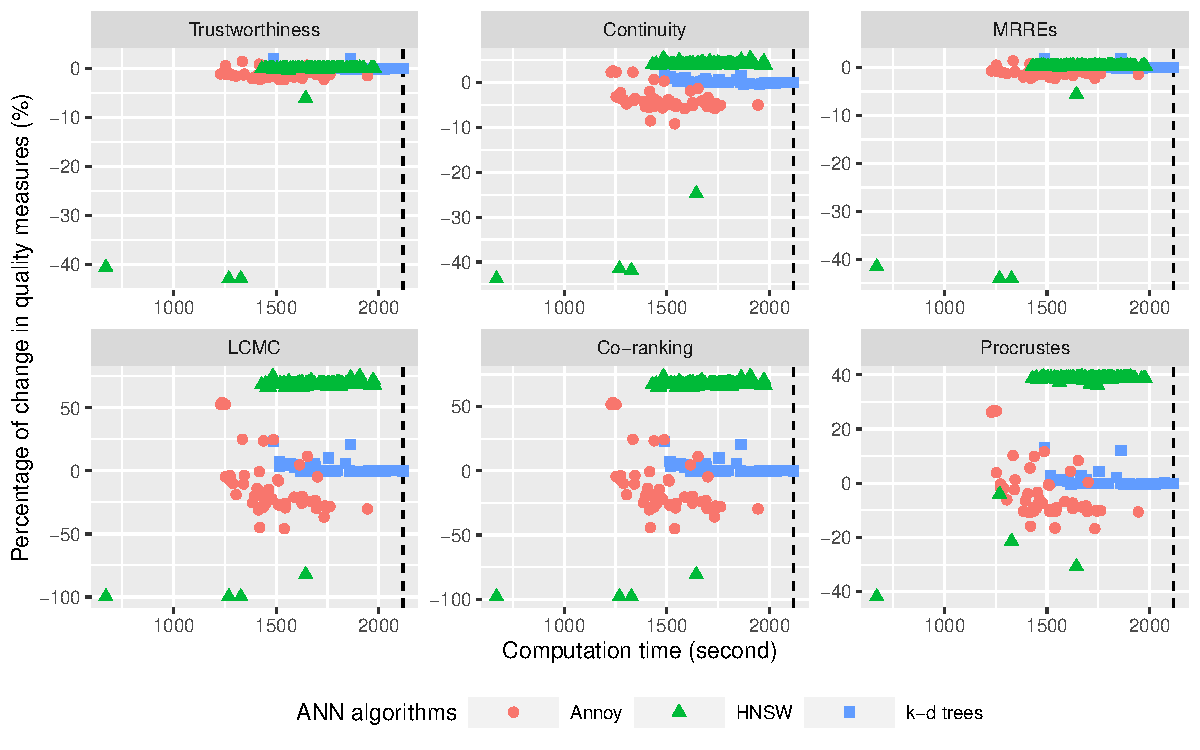
\includegraphics[width=1\linewidth]{mlann_jcgs_files/figure-latex/hllemeasure-1} 

}

\caption{Comparison of percentage change in six Hessian LLE embedding quality measures aginst computation time for three ANN methods, Annoy, HNSW and k-d trees. }\label{fig:hllemeasure}
\end{figure}

\begin{table}

\caption{\label{tab:nnmeasure}Quality measures using true nearest neighbors for four manifold learning methods. All quality measures range from 0 to 1 where higher value indicates a better embedding. }
\centering
\resizebox{\linewidth}{!}{
\begin{tabular}[t]{lrrrrrr}
\toprule
Method & Trustworthiness & Continuity & MRREs & LCMC & Co-ranking & Procrustes\\
\midrule
\textbf{Isomap} & \textbf{0.993} & \textbf{0.968} & \textbf{0.994} & \textbf{0.328} & \textbf{0.330} & \textbf{0.467}\\
LaplacianEigenmaps & 0.968 & 0.942 & 0.974 & 0.193 & 0.195 & 0.278\\
LLE & 0.950 & 0.922 & 0.964 & 0.222 & 0.224 & 0.330\\
HLLE & 0.896 & 0.863 & 0.917 & 0.105 & 0.107 & 0.196\\
\bottomrule
\end{tabular}}
\end{table}

Overall, the results from this benchmark study do seem to suggest that approximate nearest neighbors are suitable for use in manifold learning algorithms. In particular, we would recommend Annoy for the greatest computational speed up and warn that care should be taken if using HNSW due to the instability of this algorithm in a small number of cases. When using Annoy, the improvement in computational time comes at the cost of at most a small reduction in the accuracy. This result is robust to the use of different manifold learning algorithms, different measures of embedding accuracy, and different choices of tuning parameters for approximate nearest neighbor algorithms.

\hypertarget{smartmeter}{%
\section{Application to smart meter data}\label{smartmeter}}

\hypertarget{irish-smart-meter-dataset}{%
\subsection{Irish Smart meter dataset}\label{irish-smart-meter-dataset}}

Next, we consider smart-meter data for residential and non-profiled meter consumers, collected as part of a behavioral trial conducted by the Commission for Energy Regulation (CER) in Ireland (\protect\hyperlink{ref-cer2012-data}{Commission for Energy Regulation (CER) 2012}). Electricity smart meters record consumption, on a near real-time basis, at the level of individual commercial and residential properties. The CER dataset does not include energy for heating systems since it is either metered separately, or households use a different source of energy, such as oil or gas. In this study, the installed cooling systems are also not reported.

We use measurements of half-hourly electricity consumption gathered from 3,639 residential consumers over 535 consecutive days. Every meter provides electricity consumption between 14 July 2009 and 31 December 2010. Demand data from two smart meters (ID 1003 and 1539) are shown in Figure \ref{fig:smartmeter} as time-series plots. It is obvious that these meters have relatively different patterns. Meter 1539 (bottom of Figure \ref{fig:smartmeter}) has a period of around 150 days with lower (approximately half) the electricity usage of remaining days and is otherwise relatively stable. In contrast, Meter 1003 (top of Figure \ref{fig:smartmeter}) exhibits regular spikes on weekends.

\begin{figure}

{\centering 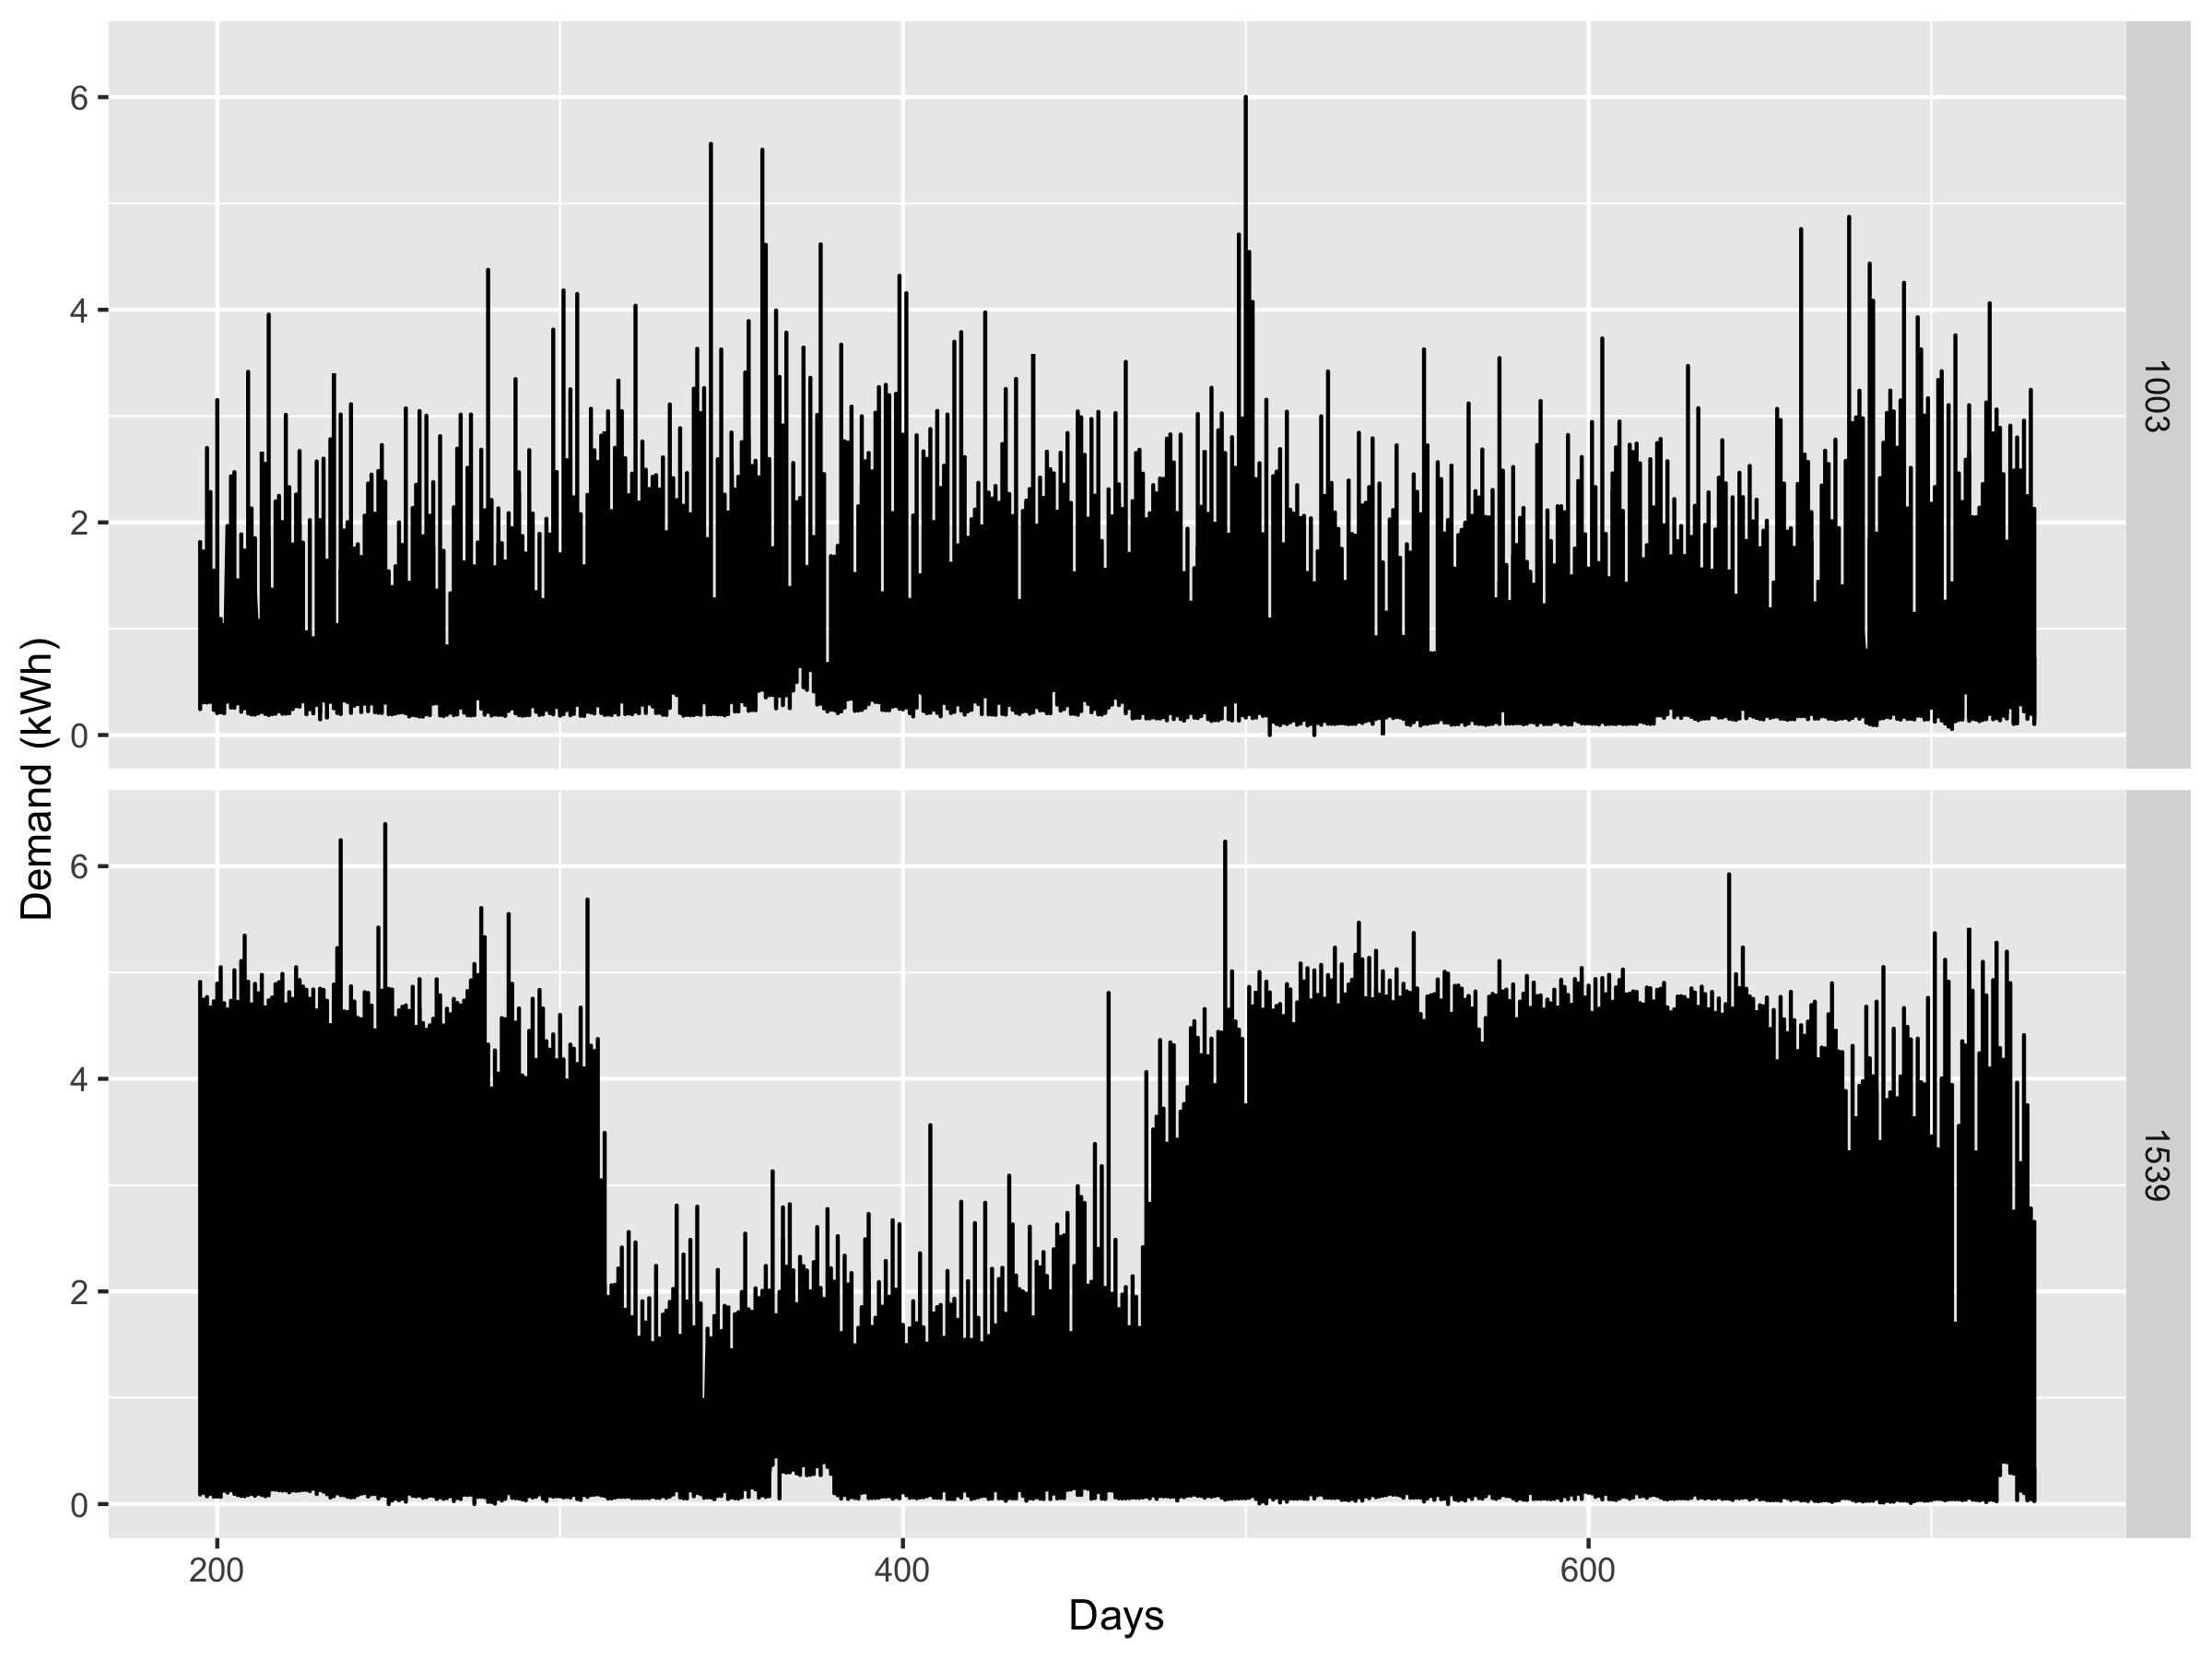
\includegraphics[width=0.8\linewidth]{/Users/fche0019/git/mlann_github/paper/figures/smartmeter} 

}

\caption{Two smart-meter demand examples, ID 1003 and ID 1539, from the Irish smart meter data set.}\label{fig:smartmeter}
\end{figure}

For electricity demand data, one particular problem of interest is to visualize and identify households or periods of the week with anomalous usage patterns. For this reason, the object of interest in comparing households or periods of the week is the distribution of electricity demand rather than the raw data itself (\protect\hyperlink{ref-Hyndman2018-ia}{R. J. Hyndman, Liu, and Pinson 2018}). An additional advantage of looking at distributions rather than raw data is that it provides a convenient mechanism for handling missing data which can be a significant problem in smart meter data applications. In the next section, we first describe how discrete approximations to the distributions of interest are computed. We then describe how the connection between popular metrics on the space of probability distributions (in particular the Hellinger and Total Variation distance) and the \(L_1\) and \(L_2\) norms of a vector containing probabilities allows us to apply manifold learning techniques on statistical manifolds.

\hypertarget{dataprocessing}{%
\subsection{Data processing}\label{dataprocessing}}

\hypertarget{estimating-empirical-distributions}{%
\subsubsection*{Estimating empirical distributions}\label{estimating-empirical-distributions}}
\addcontentsline{toc}{subsubsection}{Estimating empirical distributions}

Let \(d_{i,t}\) denote the electricity demand for observation \(i\) and for time period \(t\) (subsequently we will see that \(i\) can either index the household, time of the week, or both, while \(t\) may index the week or half-hour period). The objective is to approximate the distribution of electricity demand for observation \(i\), \(F_i\), over time. The first step is to group all data together and construct an evenly spaced grid \(\kappa_0,\kappa_1,\dots,\kappa_G\) of size \(G=200\) with \(\kappa_0=\underset{i,t}{\min} \{d_{i,t}\}\) and \(\kappa_G=\underset{i,t}{\max} \{d_{i,t}\}\) as endpoints. This provides \(200\) bins which can be used to construct a discrete distribution approximation to \(F_i\). This is found by computing \(\pi_{i,g}=(1/T)\sum_t I(\kappa_{g-1}<d_{i,t}<\kappa_g)\) where \(T\) is the total number of time periods. The resulting vector \(\pi_i\) represents a probability mass function over the discrete bins.

As an alternative, a kernel density estimate could be used. However, since the data contain a large number of zeros, a discrete distribution is more appropriate than a smooth continuous distribution. Also, the data are heavily skewed meaning that standard kernel densities may underestimate the tails of the distribution. Most importantly, an advantage of using a discrete distribution is that manifold learning algorithms with ANN can be directly applied to \(\pi_i\) or simple transformations of \(\pi_i\) in a way that either the Euclidean or Manhattan distance between such vectors will correspond to popular metrics for probability distributions.

\hypertarget{hellinger-distance-and-total-variation-distance}{%
\subsubsection*{Hellinger distance and Total Variation distance}\label{hellinger-distance-and-total-variation-distance}}
\addcontentsline{toc}{subsubsection}{Hellinger distance and Total Variation distance}

For the manifold learning algorithms discussed in Section \ref{mlann}, it is often assumed that the manifold lies in a \(p\)-dimensional ambient space. Although the approximate nearest neighbor algorithms we consider can be applied to metric spaces that are not necessarily Euclidean, they generally require that observations can be characterized as vectors in \(\mathbb{R}^p\). Therefore it may not immediately be clear how these algorithms can be applied to a statistical manifold. The key advantage of estimating the electricity usage distributions as discrete over a domain of fixed bins is that it allows each distribution to be characterized as a vector. In this case, the Euclidean distance between \(\sqrt{\pi_{i}}\) and \(\sqrt{\pi_{j}}\) where square roots are taken element-wise is equal to the Hellinger distance between our approximations to \(F_{i}\) and \(F_{j}\) (up to a constant scale). Similarly the Manhattan distance between \(\pi_{i}\) and \(\pi_{j}\) is equal to the Total Variation distance between \(\hat{F}_{i}\) and \(\hat{F}_{j}\). The Hellinger distance and Total Variation distance are popular metrics used on the space of probability distributions (\protect\hyperlink{ref-Hellinger_undated-rs}{Hellinger, n.d.}; \protect\hyperlink{ref-LeCam1973-da}{LeCam and Others 1973}) and at least locally are good approximations to the Fisher Information metric used for statistical manifolds. By exploiting this connection between \(L_1\) and \(L_2\) norms of vector representations of probability mass functions, and metrics on spaces of probability distributions, we are able to apply manifold learning algorithms to an application where the observations are probability distributions.

\hypertarget{electricityresults}{%
\subsection{Manifold learning results for single household}\label{electricityresults}}

To start with, we consider the case of a single household where each observation is a distribution corresponding to a single half-hour of the week so that each \(i\) corresponds to one of \(48 \times 7 = 336\) day-time pairs and \(t\) corresponds to a week. We choose meter ID 1003 for this purpose since it is a household with a fairly typical pattern of electricity usage. Figure \ref{fig:neighborplot} shows a nearest neighbors graphs with \(K=20\) for meter ID 1003. The left two panels are found using k-d trees with the left panel being exact (\(\varepsilon = 0\)) and the middle panel being approximate (\(\varepsilon = 1\)).
We note that the ANN output with \(\varepsilon = 1\) does not differ much from other values such as a \(\varepsilon\) of 0.5 or 2. We also use Annoy with \(\textit{n\_trees}=\textit{search\_k}=50\) to plot the corresponding nearest neighbor graph on the right panel of Figure \ref{fig:neighborplot}.
The three subplots appear quite similar to each other with a recall rate of 1 for the exact graph, 0.977 for k-d trees, and 0.992 for Annoy, suggesting that for the smart meter data, ANN techniques can be used within manifold learning to save computation time and memory without having too severe an impact on the quality of the low-dimensional representation.

\begin{figure}

{\centering \includegraphics[width=1\linewidth]{figures/knng20_1id336tow} 

}

\caption{Nearest neighborhood graphs for meter ID 1003 with $K=20$. The left subplot is the exact nearest neighborhood graph, while the middle and right subplots are the approximate ones using k-d trees ($\varepsilon = 1$) and Annoy ($\textit{n\_trees}=50$) respectively.}\label{fig:neighborplot}
\end{figure}

Since a key objective is the visualization of anomalous times of the week, Figure \ref{fig:todplot} shows \(d=2\)-dimensional representations of the data for meter ID 1003 obtained using, from left to right, Isomap, LLE, Laplacian Eigenmaps, and Hessian LLE. All cases in the top panels refer to results when exact nearest neighbors are used, while the middle and bottom panels refer to results where approximate nearest neighbors are used. The half-hour of the day that an observation belongs to is depicted using color. With the exception of LLE, the results demonstrate that similar times of day are grouped closely together. The cyclical pattern observed in the representation is indicative of the fact that low values for half-hour of the day (00:00, 00:30, 01:00) are temporally proximate to high values for half-hour of the day (22:30, 23:00, 23:30) and are therefore similar. Figure \ref{fig:todplot} also exhibits three clusters roughly corresponding to three phases of a typical day, working during the day (08:00 -- 17:00), recreation during the evening (17:00 -- 00:00), and sleeping (00:00 -- 08:00). The times of day were not explicitly used in constructing results, rather this structure was uncovered by the manifold learning algorithms themselves. This grouping is particularly prominent in Hessian LLE and to a lesser extent in Laplacian Eigenmaps. Encouragingly, all patterns are equally prominent irrespective of whether exact or approximate nearest neighbors are used.
Table \ref{tab:quality1id} also shows one of the embedding quality measures, Trustworthiness, for all the embeddings in Figure \ref{fig:todplot}. By comparing the Trustworthiness, it can be shown that using Isomap gives the highest Trustworthiness of 0.983, while Annoy leads to slightly better trustworthiness than even exact nearest neighbors. This conclusion can also be drawn for almost all the other quality measures mentioned in Section \ref{qualitymeasure}. The running times are summarised in Table \ref{tab:time1id}, with the run time for k-d trees generally shorter than Annoy except when combined with Hessian LLE. In general, the improvement from using approximate nearest neighbors relative to exact nearest neighbors is fairly minor in this example. However, we reiterate that even exact nearest neighbors here use k-d trees, compared to other methods in the literature that require all \(N^2\) pairwise distances to be computed and are thus infeasible.

\begin{figure}

{\centering 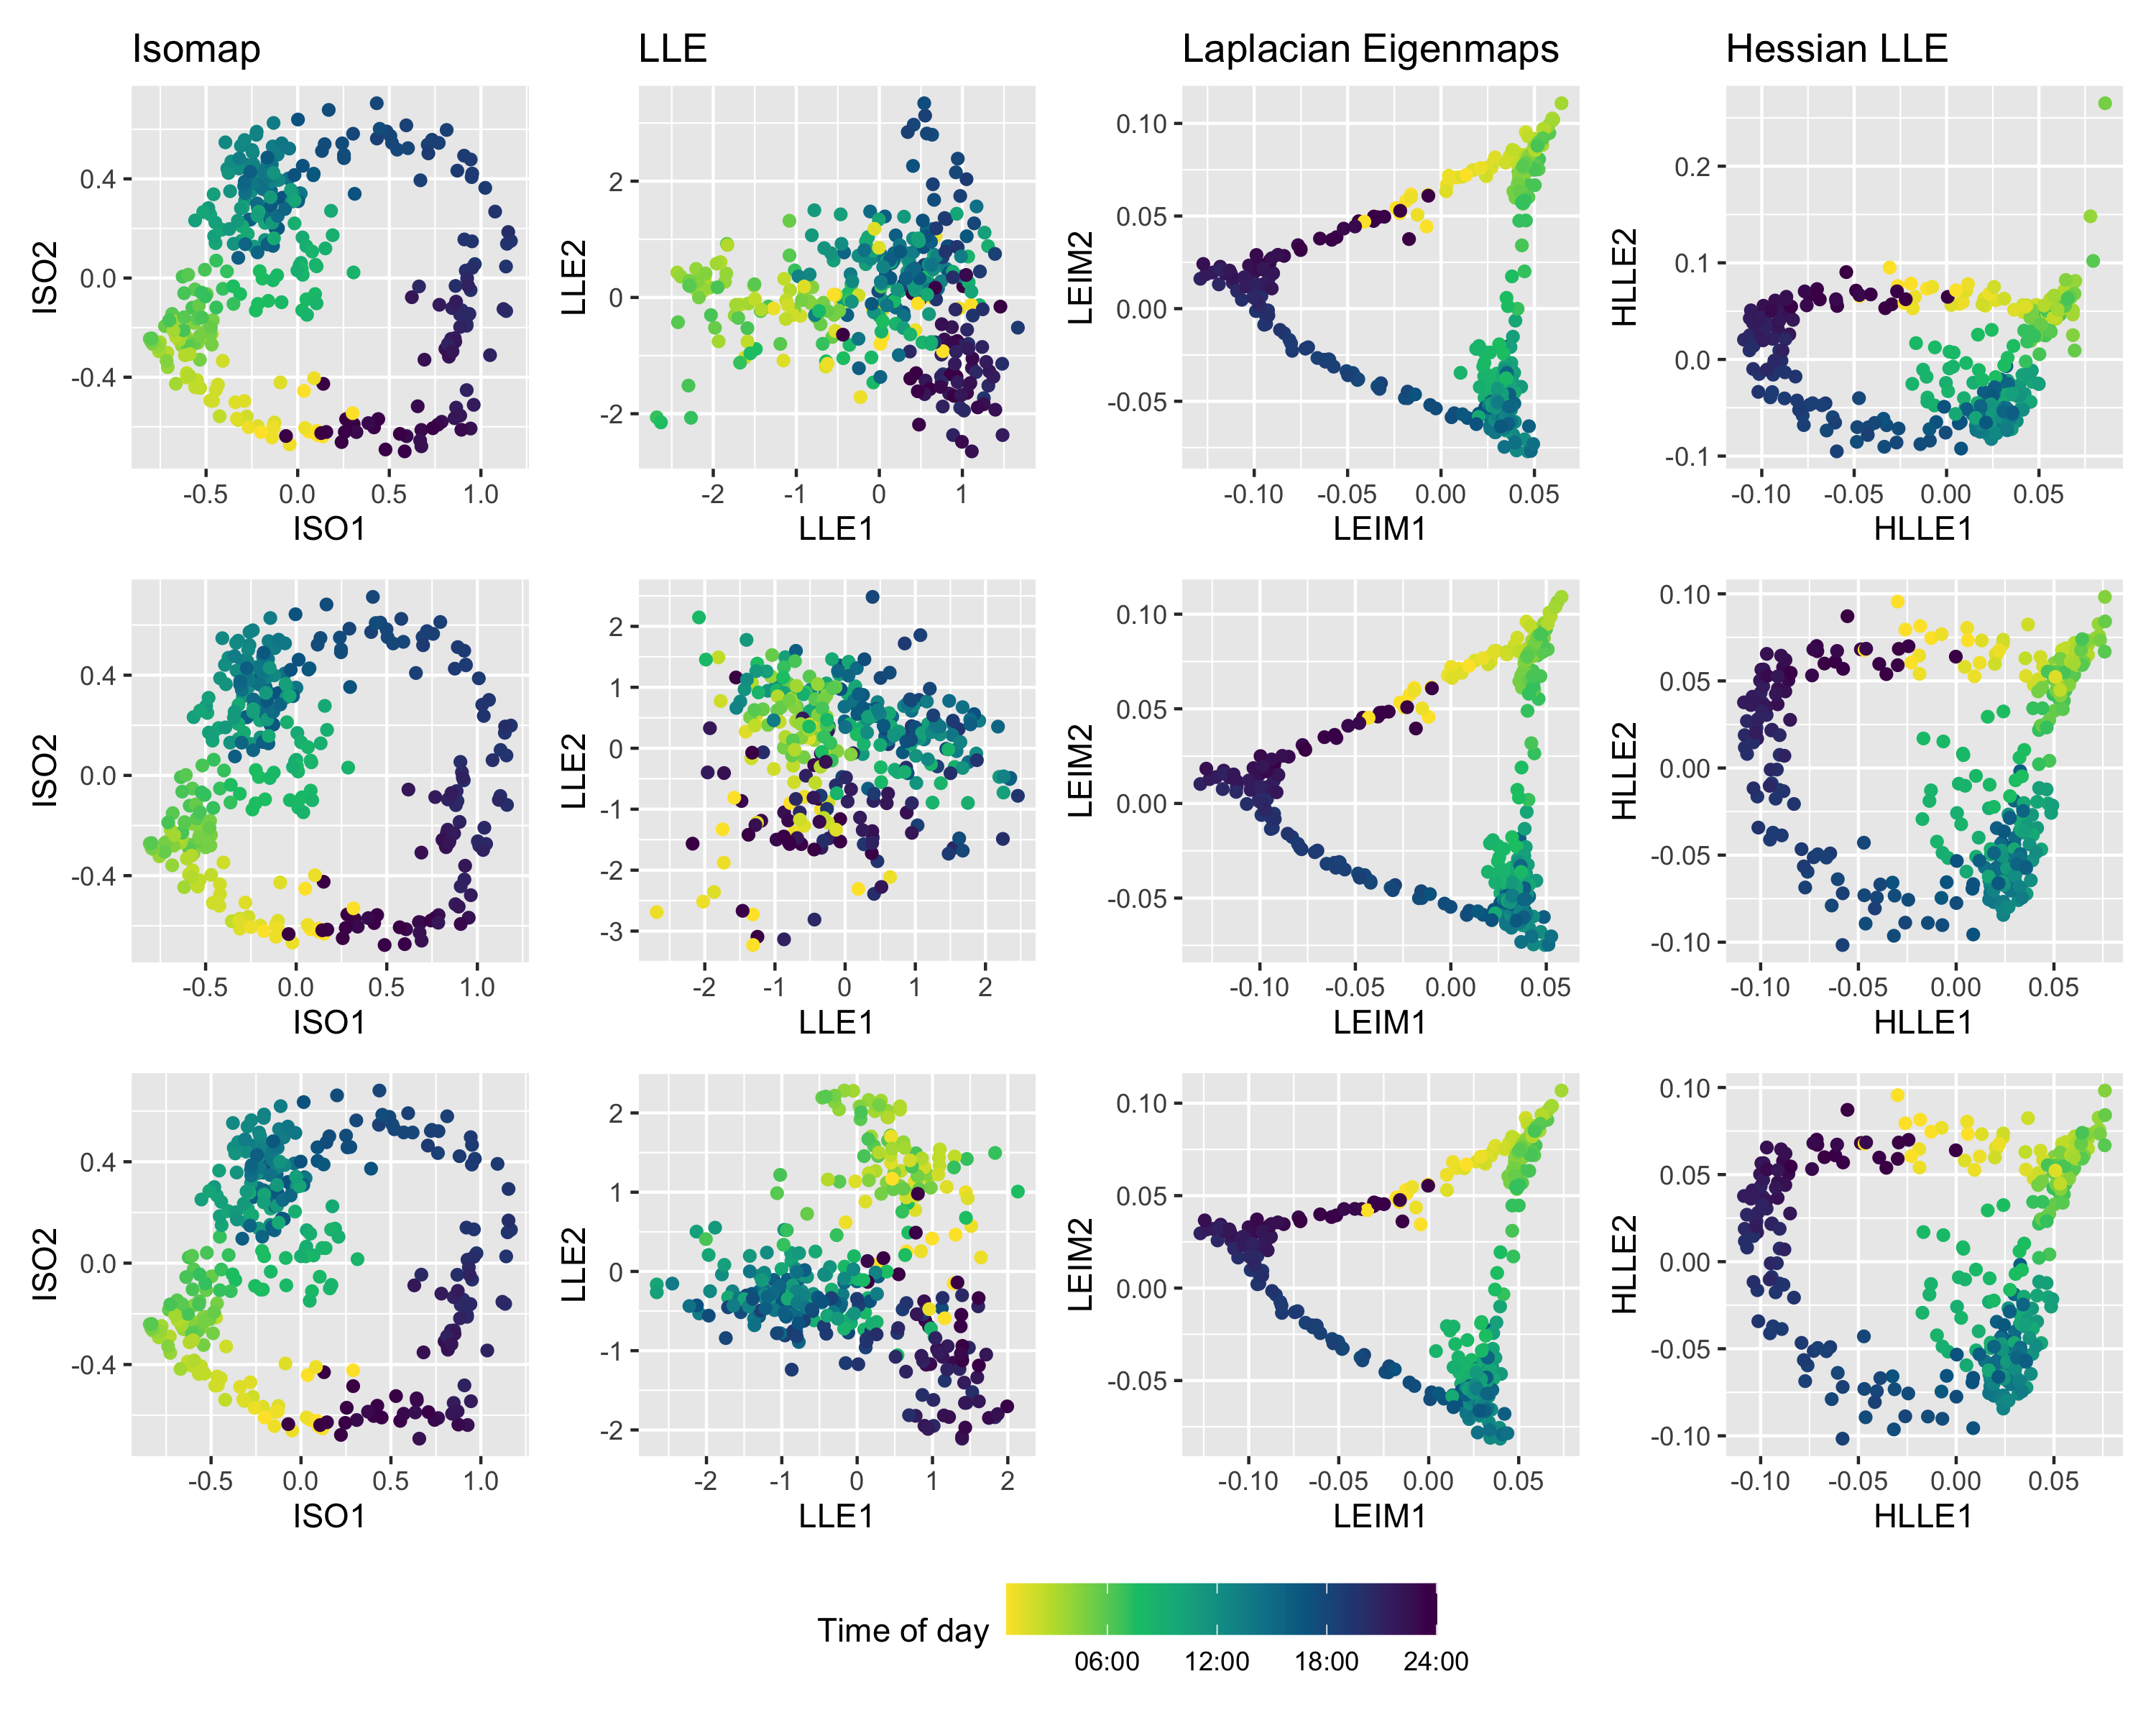
\includegraphics[width=1\linewidth]{/Users/fche0019/git/mlann_github/paper/figures/tod_compare_kdtreeannoy_1id336tow} 

}

\caption{Embeddings from four manifold learning methods (Isomap, LLE, Laplacian eigenmaps and Hessian LLE) for one household from the smart meter data. Each subplot is a scatterplot of the 2-d embedding points, with the color representing half-hourly time of the day. Top-panel: exact nearest neighbors. Middle-panel: ANN with k-d trees. Bottom-panel: ANN with Annoy.}\label{fig:todplot}
\end{figure}

\begin{table}

\caption{\label{tab:quality1id}Comparison of Trustworthiness measure using true nearest neighbors, k-d trees and Annoy for four manifold learning methods in meter ID 1003. Isomap with Annoy gives the highest Trustworthiness. }
\centering
\resizebox{\linewidth}{!}{
\begin{tabu} to \linewidth {>{\raggedright}X>{}r>{\raggedleft}X>{\raggedleft}X>{\raggedleft}X}
\toprule
  & Isomap & LLE & Laplacian Eigenmaps & Hessian LLE\\
\midrule
Exact NN & \textbf{0.983} & 0.821 & 0.937 & 0.964\\
ANN k-d trees & \textbf{0.983} & 0.756 & 0.937 & 0.966\\
\textbf{ANN Annoy} & \textbf{\textbf{0.983}} & \textbf{0.869} & \textbf{0.938} & \textbf{0.966}\\
\bottomrule
\end{tabu}}
\end{table}

\begin{table}

\caption{\label{tab:time1id}Comparison of computation time using true nearest neighbors, k-d trees, and Annoy for four manifold learning methods in meter ID 1003. Generally, k-d tree is faster than Annoy except when combined with Hessian LLE }
\centering
\resizebox{\linewidth}{!}{
\begin{tabu} to \linewidth {>{\raggedright}X>{\raggedright}X>{\raggedright}X>{\raggedright}X>{\raggedright}X}
\toprule
  & Isomap & LLE & Laplacian Eigenmaps & Hessian LLE\\
\midrule
Exact NN & 2.335 & \textbf{3.605} & 2.696 & 1.8\\
ANN k-d trees & \textbf{2.238} & 3.623 & \textbf{2.449} & 1.796\\
ANN Annoy & 2.27 & 3.859 & 2.467 & \textbf{1.77}\\
\bottomrule
\end{tabu}}
\end{table}

One particular problem of interest in visualizing smart meter data is to identify anomalous times of the week. For this reason Figure \ref{fig:anomalies1id} displays the same two-dimensional representations from using Isomap and Annoy as Figure \ref{fig:todplot} but with colors now used to demonstrate points in areas of high density using the method of \protect\hyperlink{ref-Hyndman1996-lk}{Rob J. Hyndman} (\protect\hyperlink{ref-Hyndman1996-lk}{1996}). We identify the anomalies as the observations with the 10 lowest density values and these are shown in black points with the time of week index labeled in blue. While the anomalies identified by each manifold learning algorithm differ, when the same manifold learning algorithm, Isomap, is used, the use of approximate nearest neighbors has little impact on the identified anomalies.

\begin{figure}

{\centering 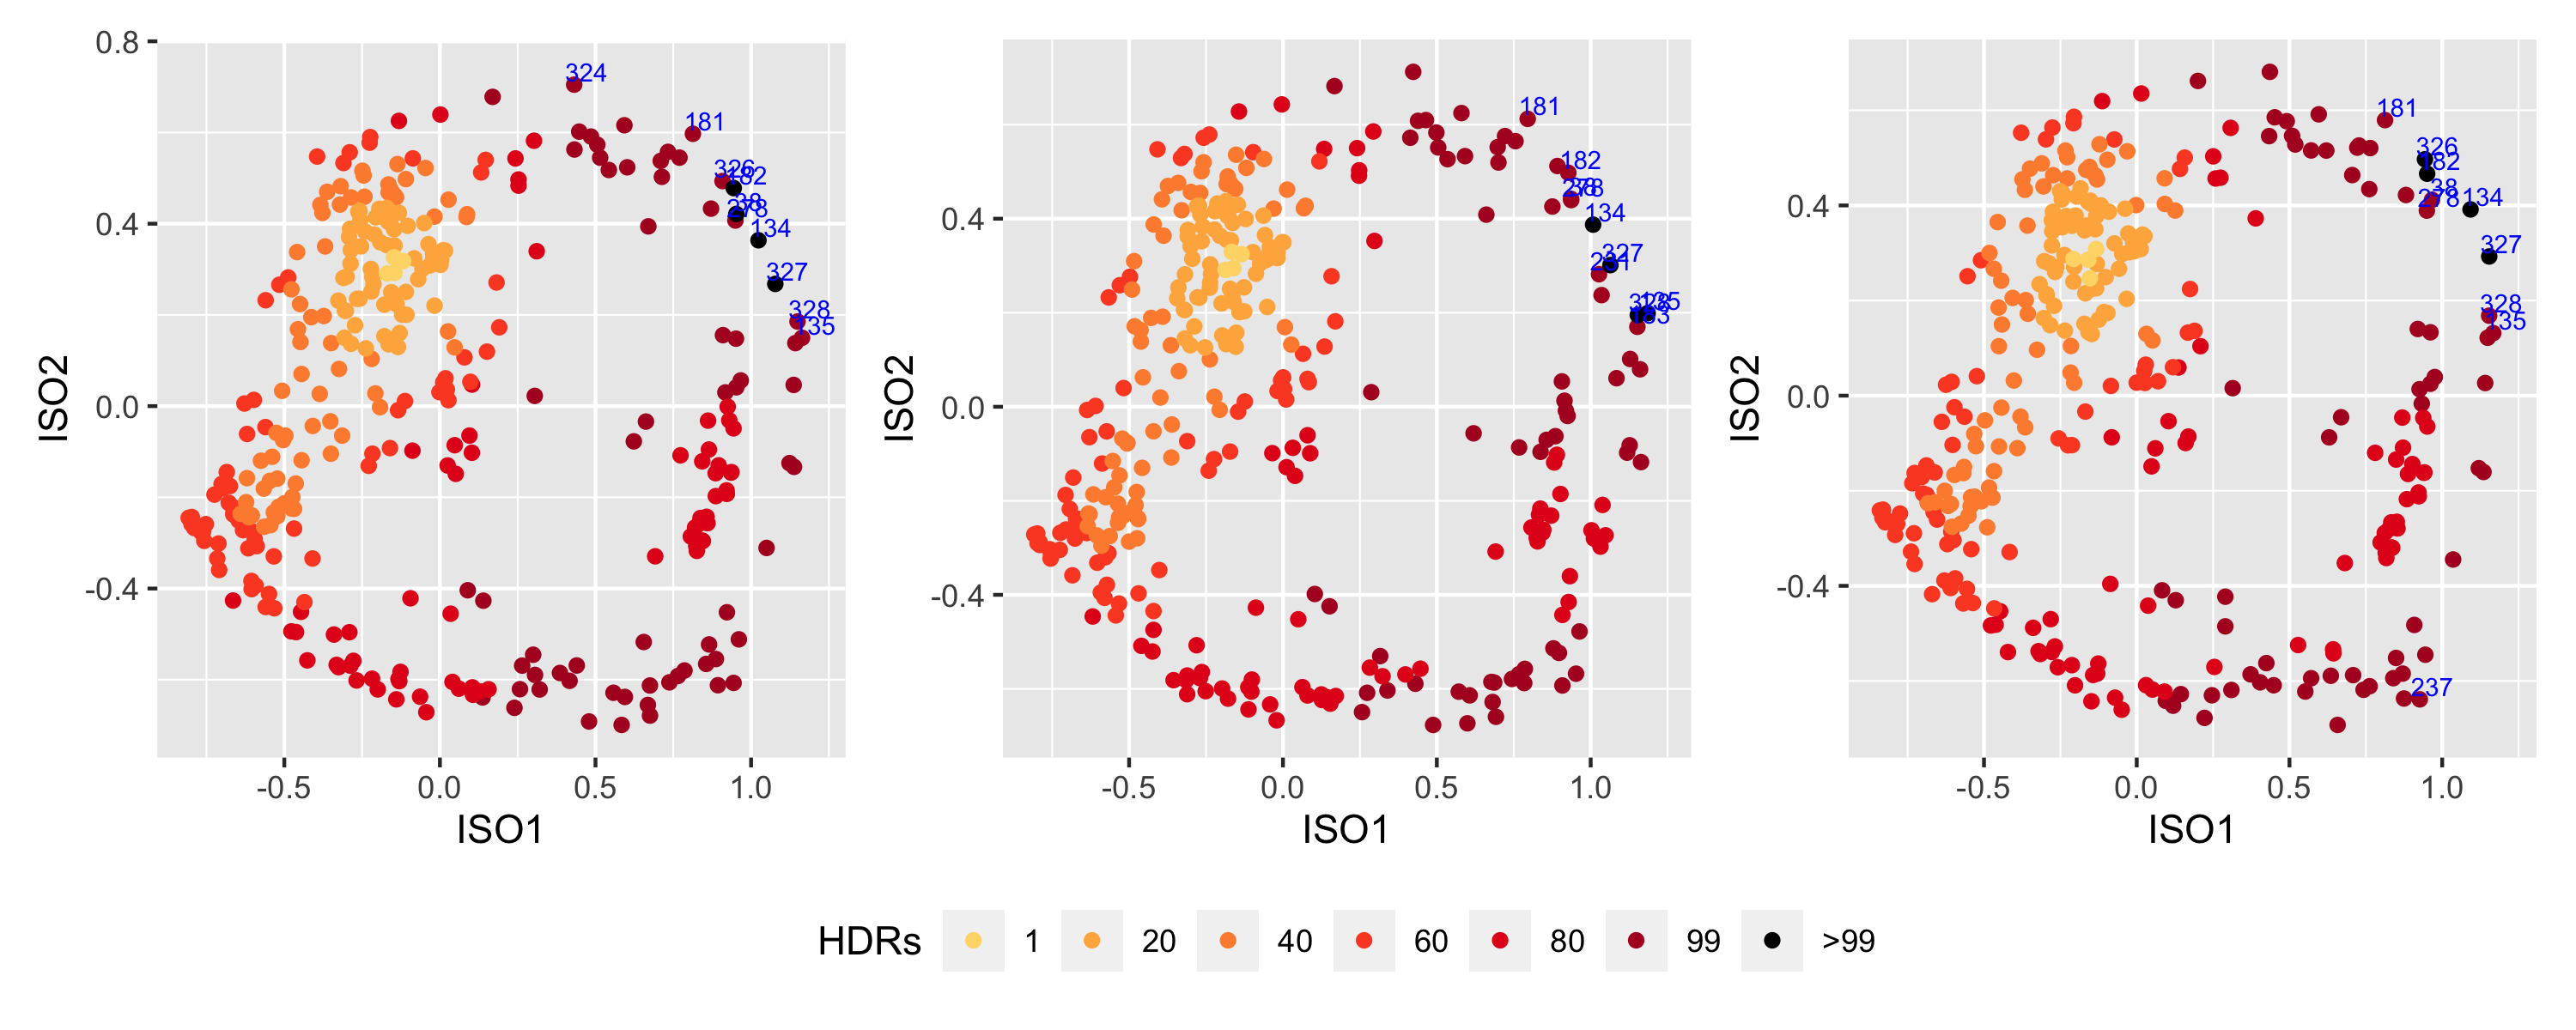
\includegraphics[width=1\linewidth]{/Users/fche0019/git/mlann_github/paper/figures/hdr10_compareisomap_kdtreeannoy_1id336tow} 

}

\caption{Highest density region plot for one household (Meter 1003) from the Isomap embeddings using exact NN (left panel), k-d trees (middle panel) and Annoy (right panel). The different colours represent highest density regions with different coverage probabilities. The most typical points (the 1\% HDR) are shown in yellow, while the top 10 most anomalous are shown in black with the time of week index in blue.}\label{fig:anomalies1id}
\end{figure}

We can gain further insight by comparing distributions corresponding to specific times of the week identified as anomalous and typical by Figure \ref{fig:anomalies1id}. In Figure \ref{fig:compare2tow}, the left two panels in orange correspond to the typical periods 134 and 317 (corresponding to Monday 12 pm and Sunday 11 am respectively), while the right two panels in black display the anomalous, periods 24 and 310 (corresponding to Wednesday 7 am and Sunday 11 pm respectively). The typical periods show relatively lower electricity usage, and the distributions and are skewed right. In contrast, for anomalous periods, electricity demand is generally higher and distributions exhibit a thicker right tail. In particular, there is a more bimodal distribution on Wednesday at 7 pm, which may suggest certain patterns of behavior are undertaken by this specific household on some but not all weeks at this time (e.g.~entertaining guests).

\begin{figure}

{\centering 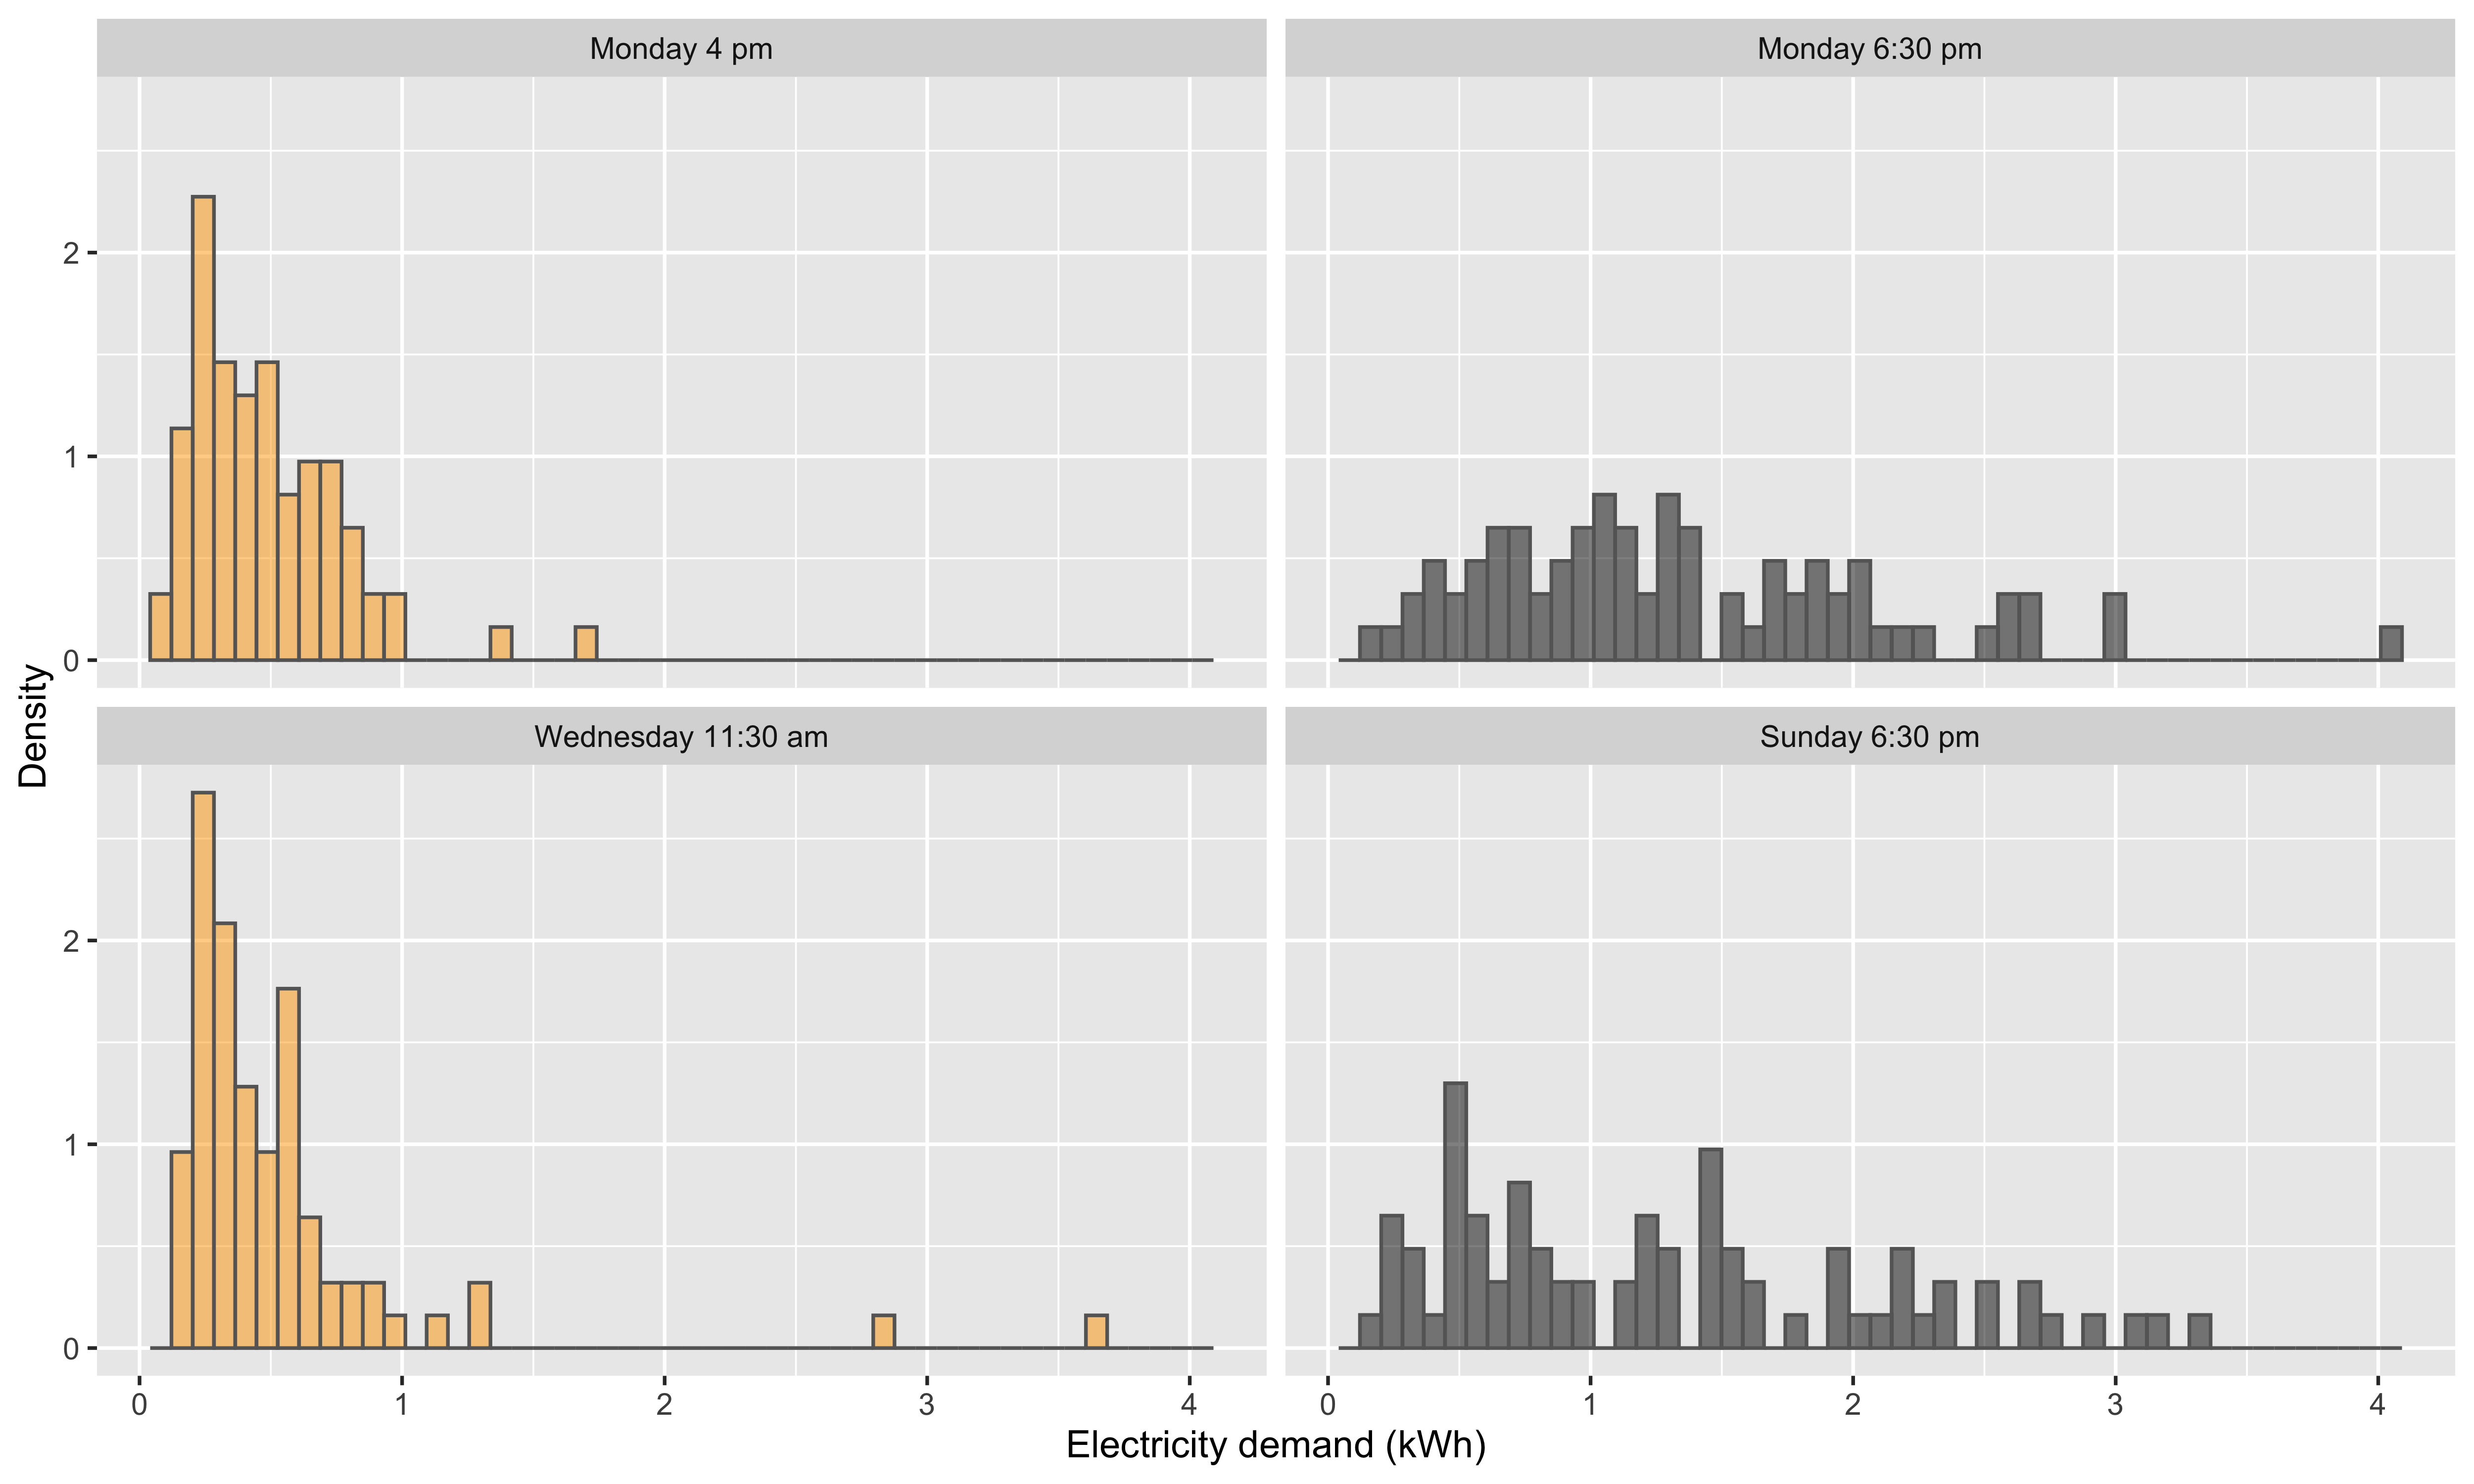
\includegraphics[width=1\linewidth]{/Users/fche0019/git/mlann_github/paper/figures/electricity_compare2tow_1id336tow} 

}

\caption{Electricity demand distribution plots for four time of week periods of meter ID 1003. The most typical periods, Monday 12pm and Sunday 11am, are shown in yellow (left panels), while the most anomalous periods, Wednesday 7pm and Sunday 11pm, are shown in black (right panels). }\label{fig:compare2tow}
\end{figure}

\hypertarget{comparison-between-households}{%
\subsection{Comparison between households}\label{comparison-between-households}}

To compare all 3,639 households in the Irish smart meter data we consider two ways to compute distances between observations. The first is to compute the density of each household's energy usage while ignoring the time of the week; using the notation of Section \ref{dataprocessing}, \(i\) corresponds to the household and \(t\) corresponds to the half-hour period. However, since the time of week is highly informative in electricity consumption data, an alternative would be to compute densities such that the index \(i\) corresponds to a household/time-of-week pair and index \(t\) corresponds to the week. In this case, we use \(F_{j,h}\) to denote the distribution corresponding to household \(j\) and time of week \(h\), and \(\pi_{j,k}\) to denote a vector whose entries give values of a probability mass function of a discrete approximation to \(F_{j,h}\). The distance between household \(j\) and household \(k\) can then be computed as
\begin{equation}\label{eq:betweenhhmetric}
  \delta_{j,k}=\sum\limits_{h=1}^{336}d(F_{j,h},F_{k,h}),
\end{equation}
where \(d(.,.)\) is the total variation metric between two discrete distributions. This metric resembles that used by \protect\hyperlink{ref-Hyndman2018-ia}{R. J. Hyndman, Liu, and Pinson} (\protect\hyperlink{ref-Hyndman2018-ia}{2018}) who use a sum of Jenson-Shannon divergences rather than the total variation metric. However, an important advantage of using the total variation metric is that the \(\delta_{j,k}\) is equivalent to a Manhattan distance between the stacked vectors \(\pi_j=(\pi'_{j,1},\ldots,\pi'_{j,336})'\) and \(\pi_k=(\pi'_{k,1},\ldots,\pi'_{k,336})'\). Unlike \protect\hyperlink{ref-Hyndman2018-ia}{R. J. Hyndman, Liu, and Pinson} (\protect\hyperlink{ref-Hyndman2018-ia}{2018}), we do not have to compute all pairwise distances (an \(O(n^2)\) operation) before computing nearest neighbors; instead, we can compute exact nearest neighbors using k-d trees or, in an even faster time, approximate nearest neighbors.

Similar to the single household case in Section \ref{electricityresults}, exact nearest neighbors is implemented by setting \(\varepsilon=0\) in k-d trees and approximate nearest neighbor is implemented using k-d trees with \(\varepsilon=1\) and Annoy with \(\textit{n\_trees}=50\). The distance metric between households is defined as in Equation \eqref{eq:betweenhhmetric}. The recall rates for these three methods are 1, 0.892, 0.994 respectively. For each scenario, the same four manifold learning algorithms are used as in Section \ref{electricityresults}. The highest density region plots of the embeddings are shown in Figure \ref{fig:allidhdr} with exact nearest neighbors on the top panel, ANN with k-d trees on the middle panel, and ANN with Annoy bottom panel. Also, the trustworthiness measure is computed for all combinations of manifold learning and nearest neighbor algorithms with results summarized in Table \ref{tab:allidmeasure}, and the corresponding computation time is reported in Table \ref{tab:allidtime}.

Isomap and Laplacian Eigenmaps are highly robust to the use of approximate nearest neighbors with the trustworthiness measures equivalent across all nearest neighbor algorithms to the third decimal place. Once again, Isomap yields the most accurate embedding according to the trustworthiness metric. Results are similar if other accuracy metrics are used. The households identified as anomalous do not change for Isomap and Laplacian Eigenmaps when approximate nearest neighbors are used. For the LLE and Hessian LLE, the trustworthiness and the identified anomalies do change across different ANN methods, however, the differences are minor. The Hessian LLE embedding has the lowest trustworthiness measure which may explain why it appears to exhibit some degeneracy in Figure \ref{fig:allidhdr}. An alternative explanation for the poor performance of Hessian LLE is that Hessian LLE is predicated on the existence of an isometric \(d\)-dimensional embedding, and for this specific dataset such an isometry may not exist for \(d=2\). As was the case in Section \ref{electricityresults}, whether the focus is upon the identification of anomalies or the trustworthiness measure, the impact of using different approximate nearest neighbor algorithms is insubstantial when compared to the choice of the manifold learning algorithm. However, in contrast to the earlier results, Table \ref{tab:allidtime} shows that a computational speedup is only observed when an approximate version of k-d trees is used and not for Annoy. This may be due to the fact that the discrete approximation is to a multivariate density and hence has a higher dimensionality. Annoy is generally recommended for data with a moderately high dimension of a few hundred to a few thousand.

\begin{figure}

{\centering 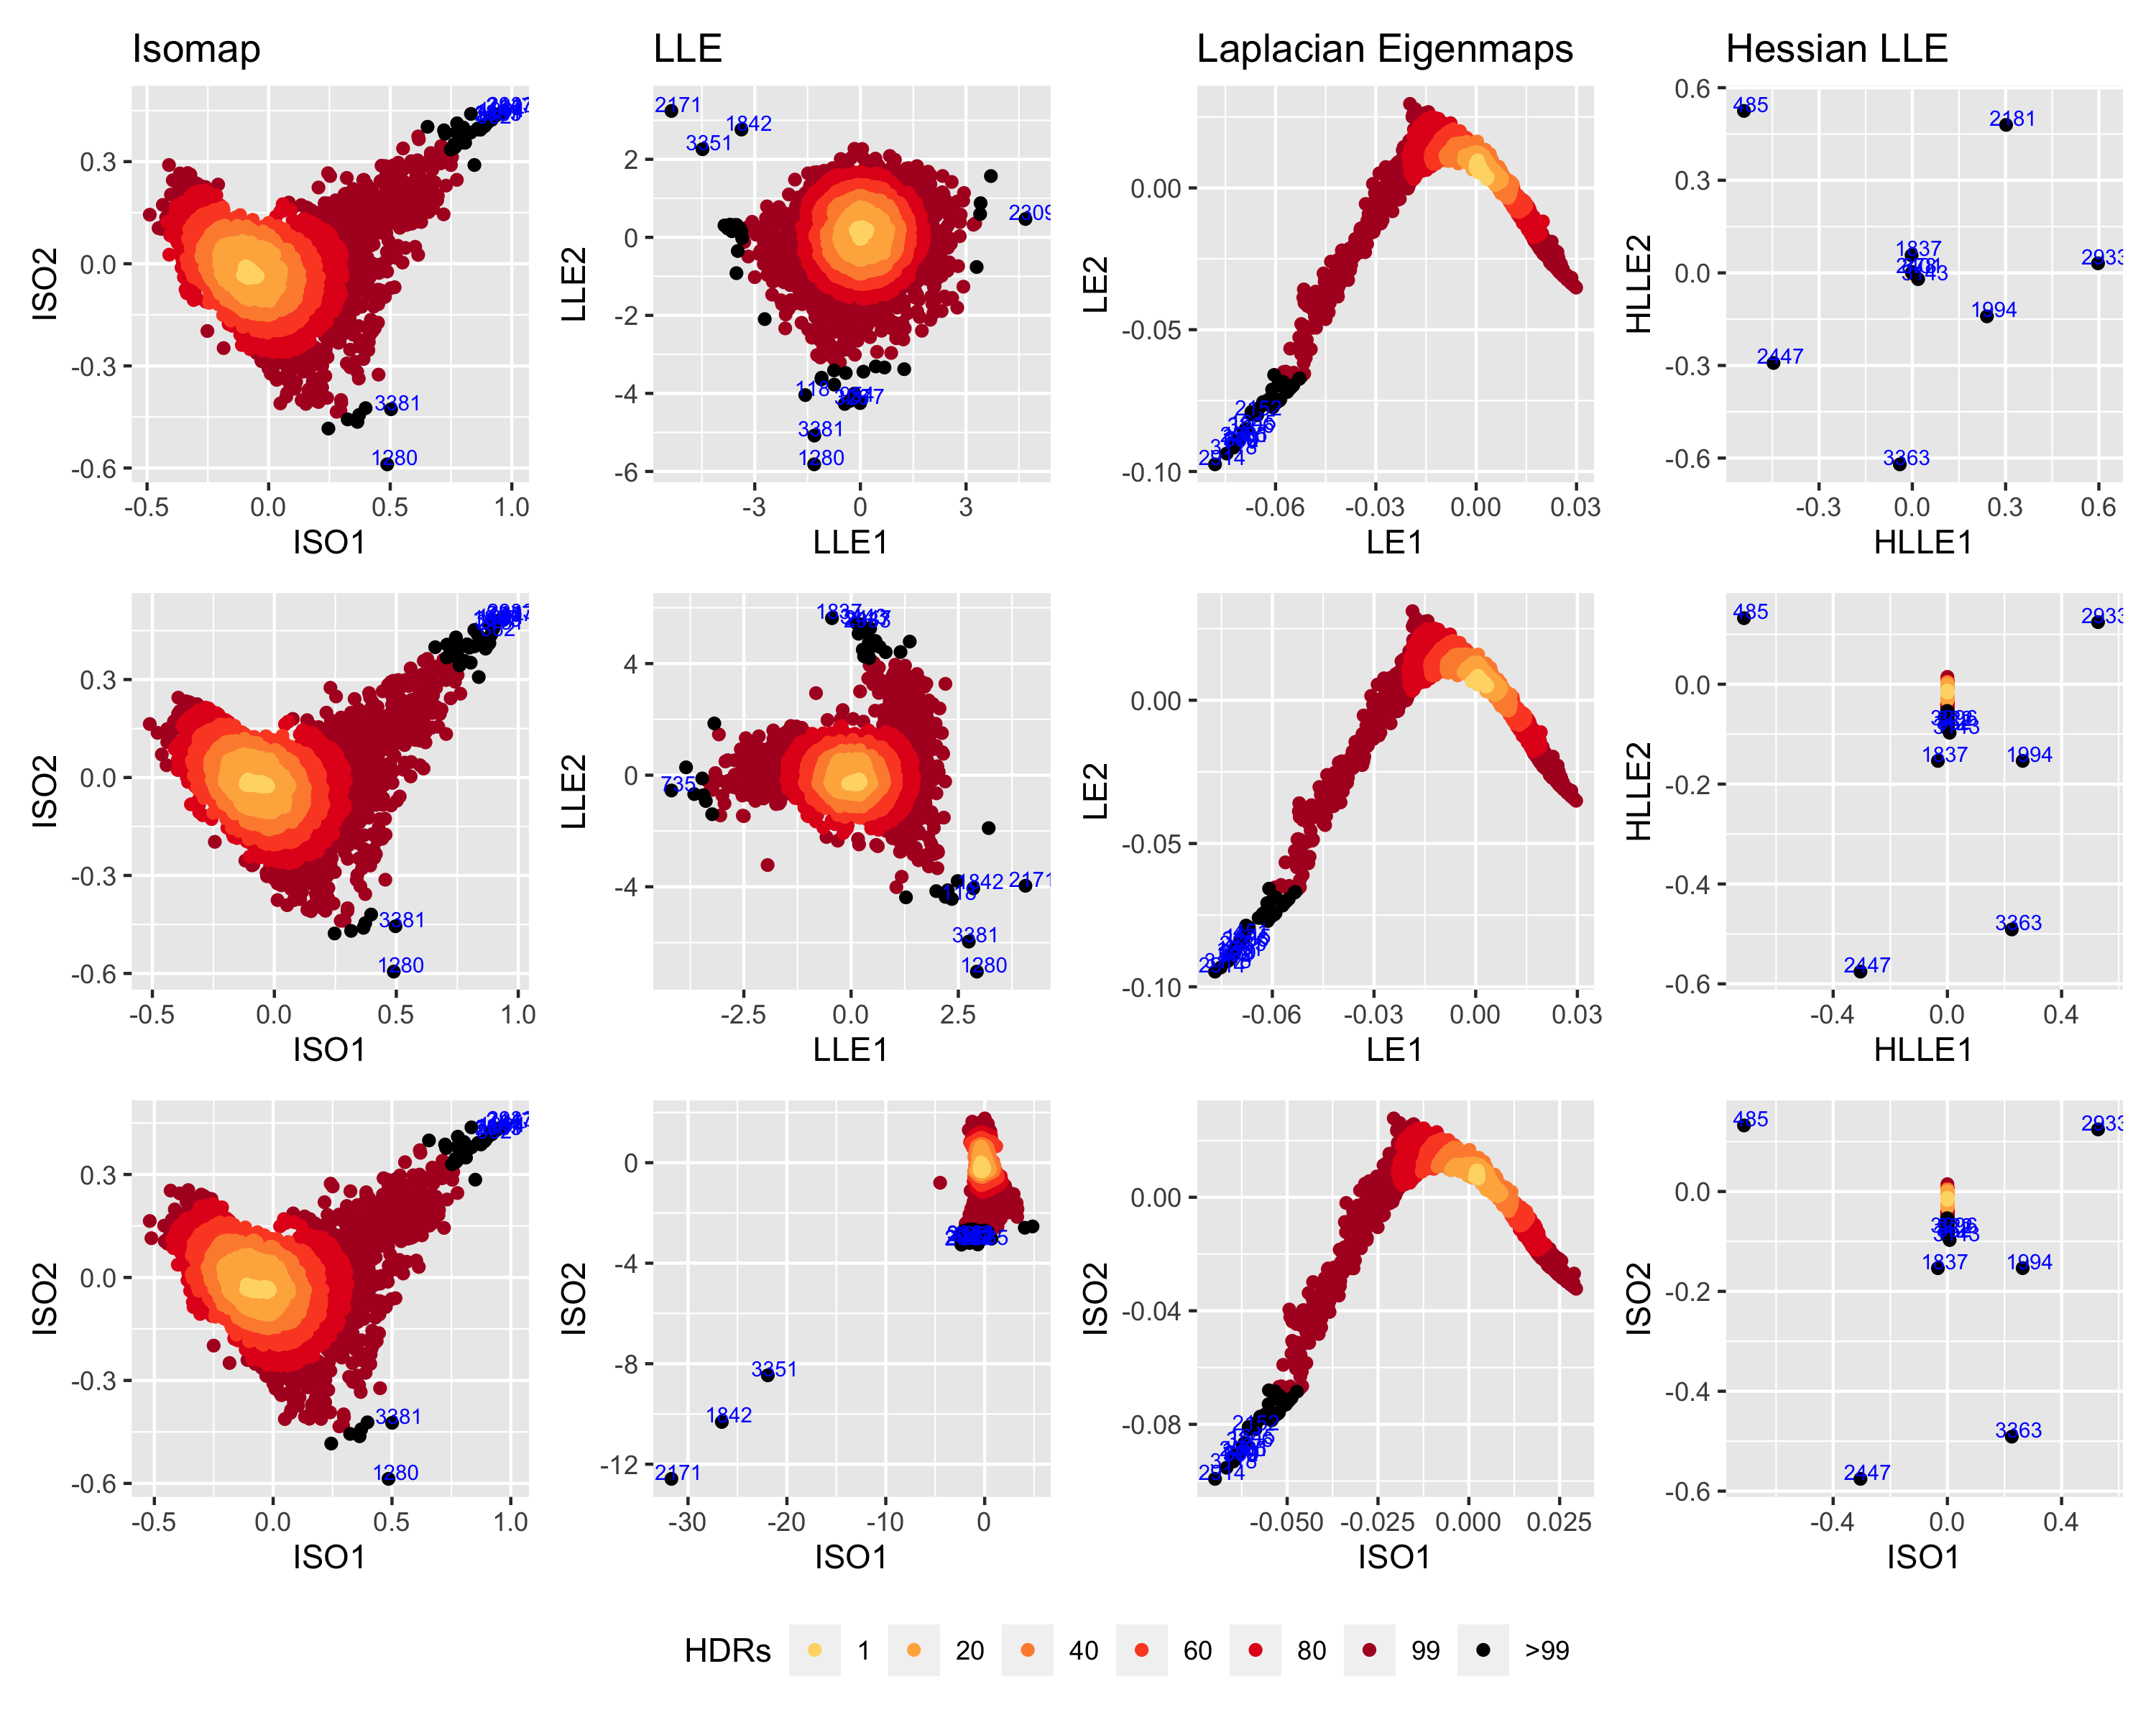
\includegraphics[width=1\linewidth]{/Users/fche0019/git/mlann_github/paper/figures/hdr10_compare4ml_kdtreeannoy_allids_nt50_3639id_notow_201length} 

}

\caption{Highest density region plots from four manifold learning methods for all 3,639 households, with each point representing the distribution of one household. Top row: exact nearest neighbors. Middle row: ANN with k-d trees. Bottom row: ANN with Annoy.}\label{fig:allidhdr}
\end{figure}

\begin{table}

\caption{\label{tab:allidmeasure}Comparison of Trustworthiness measure for all household embeddings using true nearest neighbors, k-d trees, and Annoy for four manifold learning methods. Isomap gives the highest Trustworthiness while Hessian LLE gives the lowest. }
\centering
\resizebox{\linewidth}{!}{
\begin{tabu} to \linewidth {>{\raggedright}X>{}r>{\raggedright}X>{\raggedright}X>{\raggedright}X}
\toprule
  & Isomap & LLE & Laplacian Eigenmaps & Hessian LLE\\
\midrule
Exact NN & \textbf{0.985} & \textbf{0.969} & 0.957 & 0.886\\
ANN k-d trees & \textbf{0.985} & 0.933 & 0.957 & \textbf{0.919}\\
ANN Annoy & \textbf{0.985} & 0.947 & \textbf{0.957} & 0.919\\
\bottomrule
\end{tabu}}
\end{table}

\begin{table}

\caption{\label{tab:allidtime}Comparison of computation time for all household embeddings using true nearest neighbors, k-d trees, and Annoy for four manifold learning methods. Laplacian Eigenmaps with k-d trees saves the most computation time while Annoy is the slowest. }
\centering
\resizebox{\linewidth}{!}{
\begin{tabu} to \linewidth {>{\raggedright}X>{\raggedright}X>{\raggedright}X>{\raggedright}X>{\raggedright}X}
\toprule
  & Isomap & LLE & Laplacian Eigenmaps & Hessian LLE\\
\midrule
Exact NN & 2147.908 & 2841.332 & 2046.851 & 4732.669\\
ANN k-d trees & \textbf{2075.954} & \textbf{2760.93} & \textbf{1976.831} & \textbf{4731.36}\\
ANN Annoy & 6925.794 & 6911.878 & 6203.974 & 4737.04\\
\bottomrule
\end{tabu}}
\end{table}

Further insights are gained by comparing the electricity demand distributions of typical and anomalous households. For example, in the Isomap highest density region plot, the meter IDs 3243 and 4669, are both detected as anomalies. However, they lie far away from one other in the embedding plot, suggesting that while both are anomalous, their distributions are quite different. We can compare these to one typical household, namely the household ID 1321). In Figure \ref{fig:compare3ids}, the electricity usage data of these three households are plotted over all trial days, while the corresponding quantile region plots of electricity demand by half-hour and day of the week are given in Figure \ref{fig:hdrboxplot3ids}. For all three households, the time of the week patterns are revealed in the top panel of Figure \ref{fig:hdrboxplot3ids}. When compared to the typical household 1321, the electricity demand of the anomalous households is much lower. The highest density region boxplots show that the distributions of the two anomalous households, 3243 and 4669 are quite different from each other, which is consistent with their far apart locations in the embedding plots. For household 3243, in most of the days, the electricity demand is below 1 kWh per day indicating that there are not many electrical applicants in this household or that people are away for most of the trial days, which also explains some spikes in certain days. The situation is quite different for household 4669 where for most of the time the electricity usage is below 2 kWh per day and there are certain periods with almost no usage. This shows that this household might have vacations for holidays and leave only the necessary electrical applicants on while not at home. These findings show that the manifold learning with approximate nearest neighbors works well in finding anomalous households in the smart meter data despite the large volume of data.

\begin{figure}

{\centering 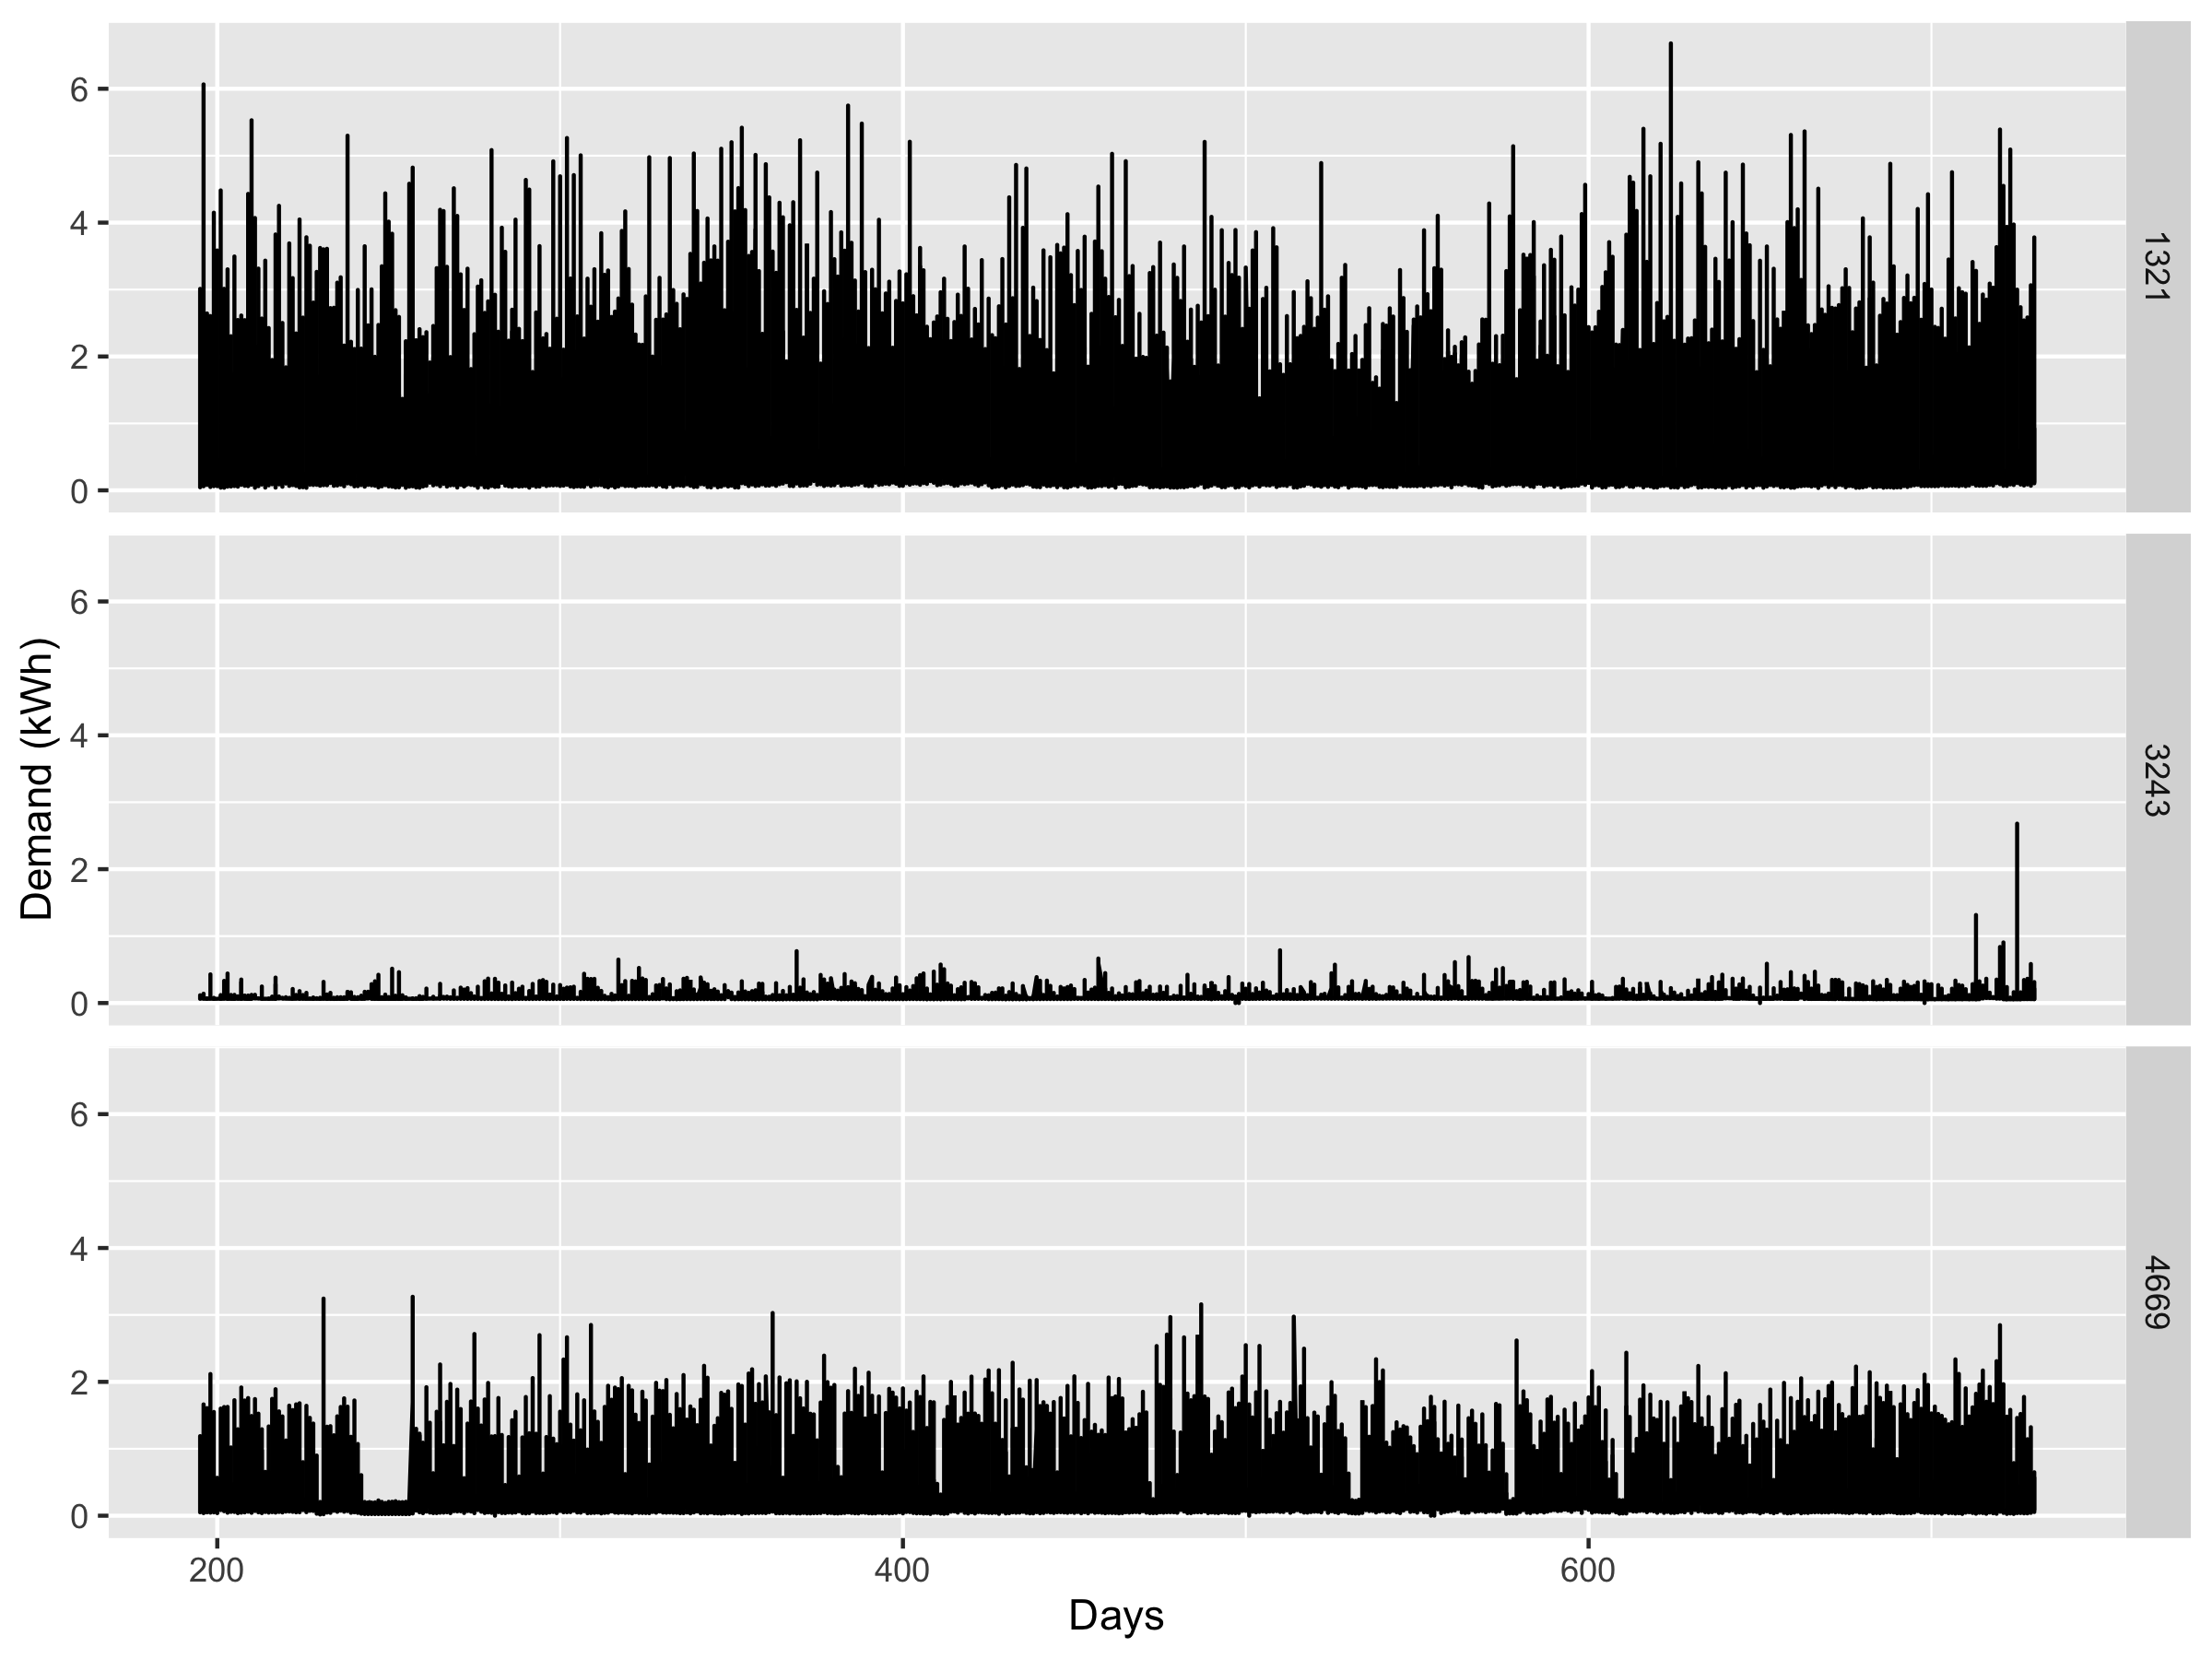
\includegraphics[width=0.8\linewidth]{/Users/fche0019/git/mlann_github/paper/figures/electricity_compare3id} 

}

\caption{Electricity demand plots of all 535 days for one typical household 1321 and two anomalies, 3243 and 4699. }\label{fig:compare3ids}
\end{figure}
\begin{figure}

{\centering 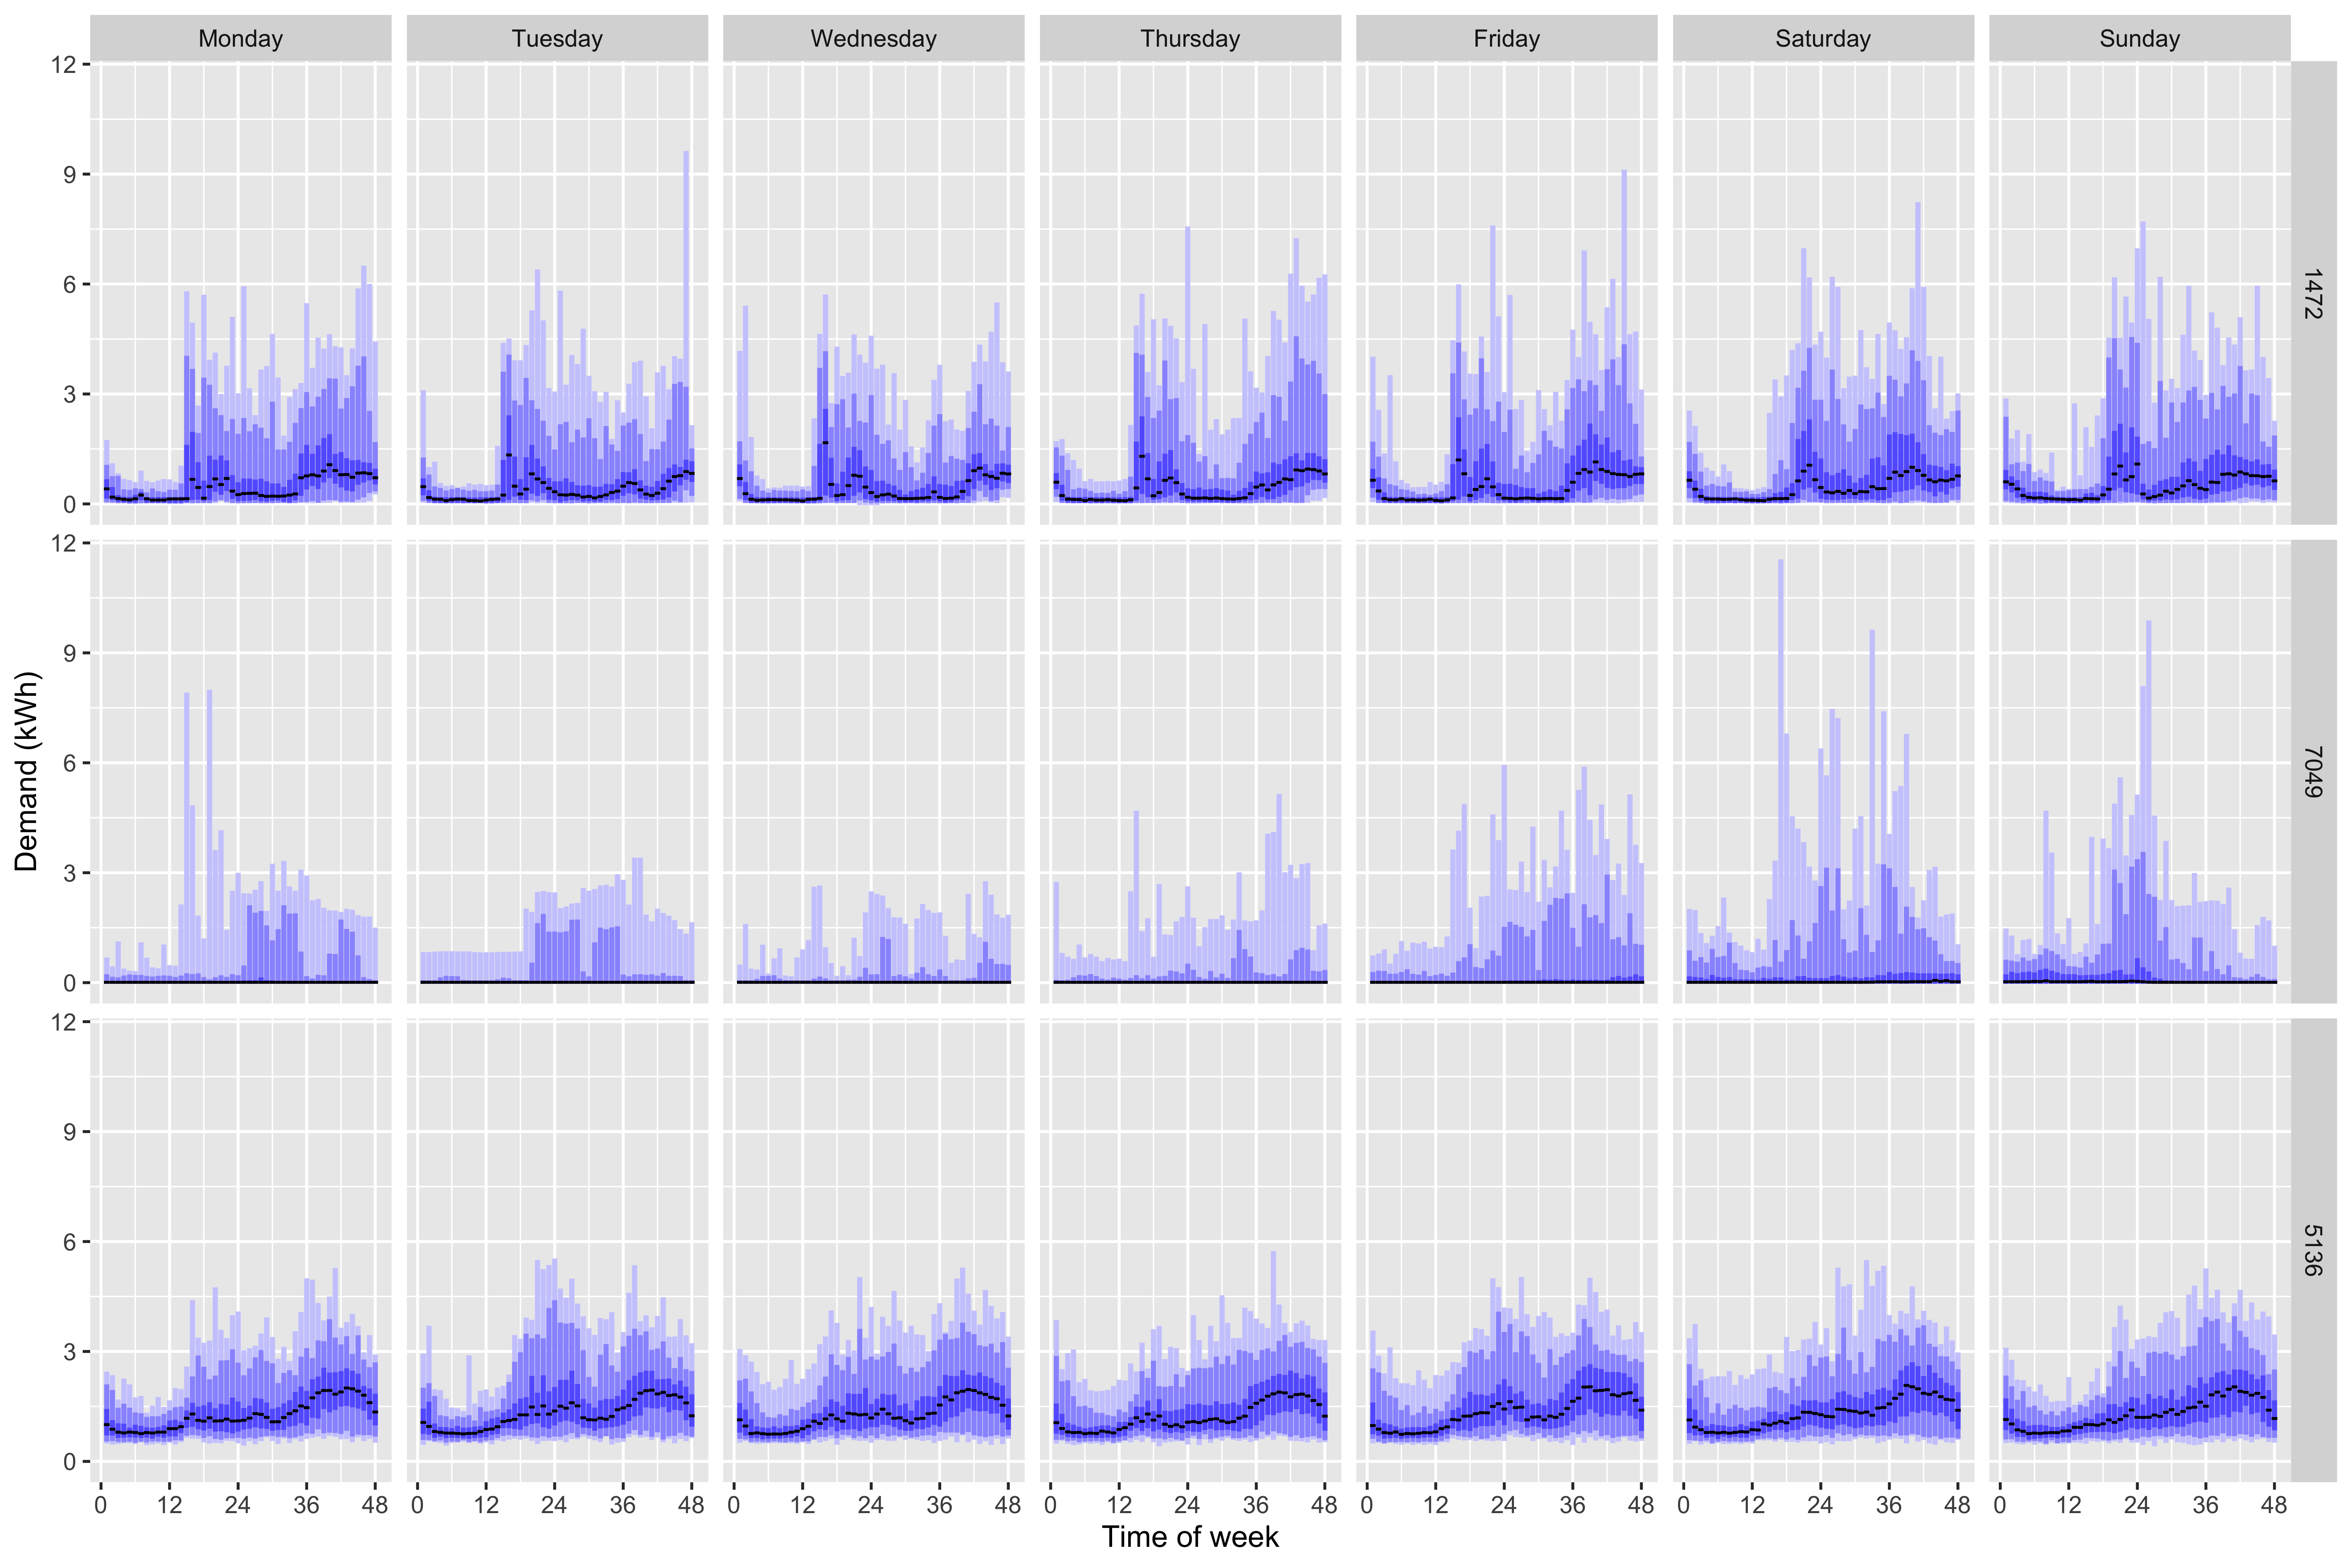
\includegraphics[width=1\linewidth]{/Users/fche0019/git/mlann_github/paper/figures/electricity_hdrbox_3id_7dow} 

}

\caption{Quantile region plots of electricity demand against the time of week for one typical household 1321 and two anomalies, 3243 and 4699. The quantile regions displayed in the plot are 99.0\%, 95.0\%, 75\%, and 50\%. }\label{fig:hdrboxplot3ids}
\end{figure}

\hypertarget{conclusion}{%
\section{Conclusions}\label{conclusion}}

In this paper, we propose the use of a broad range of approximate nearest neighbors in manifold learning algorithms to attain a lower-dimensional embedding of the high-dimensional data. By applying different combinations of manifold learning algorithms (Isomap, LLE, Laplacian Eigenmaps, and Hessian LLE) and approximate nearest neighbor methods (k-d trees, Annoy, and HNSW) to the benchmark MNIST data of handwritten digits, we show that the use of ANN methods significantly reduces computational time while maintaining a high level of embedding quality across a range of accuracy measures (LCMC, Trustworthiness \& Continuity, MRREs, Co-ranking matrix, and Procrustes measure). Annoy gives the greatest reduction in computation time --- almost four-fold when applied to Laplacian Eigenmaps. While HNSW generally achieves a high recall rate, it can return very inaccurate results in a small number of instances which in turn leads to poor embedding quality. Consequently, we recommend using Annoy or k-d trees together with manifold learning algorithms.

We also explore the electricity usage patterns of different time periods and households in the Irish smart meter dataset. In this case, the elements of the manifold in question are probability distributions. Here we propose a solution that exploits the connection between the Hellinger and Total Variation Metric used to describe the distance between discrete probability distributions and the L2 and L1 norm where the vectors are values of probability mass functions. In doing so, rather than compute all pairwise Hellinger or Total Variation distances, k-d trees and Annoy can be used to reduce computational time.
Once again, we show that ANN techniques can be used within manifold learning to save computation time and memory without having a severe impact on the quality of the low-dimensional representations. For the particular dataset, Isomap together with k-d trees gives the best tradeoff between embedding quality and computational time, while Annoy breaks down for one example that is particularly high-dimensional. Using the highest density region plots, we show how the techniques developed can successfully identify both typical and anomalous times of week and households.

There are several open questions to be explored. The first involves the selection of tuning parameters for the approximate nearest neighbor algorithm. The optimal choice may depend on a number of considerations, for instance, if manifold learning is used to detect anomalies in an online fashion, then the tuning parameters may be constrained in a way that approximate nearest neighbors are found within a certain time frame (\protect\hyperlink{ref-Talagala2020-ck}{Talagala et al. 2020}). Alternatively, tuning parameters may be selected so that a maximal level of embedding quality is achieved, where embedding quality is measured using one of the metrics we discussed in Section \ref{qualitymeasure}.

Finally, there remain a number of open issues in manifold learning including the choice of intrinsic dimension \(d\) and the choice of manifold learning algorithm itself. In the case of the former, we present results in Section \ref{smartmeter} based only on \(d=2\) due to our emphasis on visualizations and the ease of using scatter plots. However, in principle, larger values of \(d\) could be used and if visualization is required, the embedding dimensions could be summarized using principal components or using projection pursuit methods with random tours (\protect\hyperlink{ref-Cook1995-jx}{Cook et al. 1995}; \protect\hyperlink{ref-Laa2020-qx}{Laa, Cook, and Valencia 2020}). Regarding the choice of the manifold learning algorithm, we have seen that this has a much bigger impact on accuracy measures than the use of approximate nearest neighbors. This does bring into focus the need for further work on the selection of manifold learning algorithms. However, it is an encouraging result for the use of ANN which across a wide range of algorithms improves the computational speed of manifold learning.

\hypertarget{acknowledgment}{%
\section*{Acknowledgment}\label{acknowledgment}}
\addcontentsline{toc}{section}{Acknowledgment}

This research was supported in part by the Monash eResearch Centre and eSolutions-Research Support Services through the use of the MonARCH HPC Cluster.
We would also like to acknowledge the support of the \emph{Australian Research Council (ARC) Centre of Excellence for Mathematical and Statistical Frontiers (ACEMS)} for this project.

\hypertarget{supplementary-materials}{%
\section*{Supplementary Materials}\label{supplementary-materials}}
\addcontentsline{toc}{section}{Supplementary Materials}

The GitHub repository, \url{https://github.com/ffancheng/paper-mlann}, contains all materials required to reproduce this article. The code and data files are also available online in the same repository.

\hypertarget{references}{%
\section*{References}\label{references}}
\addcontentsline{toc}{section}{References}

\hypertarget{refs}{}
\begin{CSLReferences}{1}{0}
\leavevmode\hypertarget{ref-Amari2016-hk}{}%
Amari, Shun-Ichi. 2016. \emph{Information Geometry and Its Applications}. Springer.

\leavevmode\hypertarget{ref-Arya1998-bv}{}%
Arya, Sunil, David M Mount, Nathan S Netanyahu, Ruth Silverman, and Angela Y Wu. 1998. {``An Optimal Algorithm for Approximate Nearest Neighbor Searching Fixed Dimensions.''} \emph{Journal of the ACM} 45 (6): 891--923.

\leavevmode\hypertarget{ref-Aumuller2020-nk}{}%
Aumüller, Martin, Erik Bernhardsson, and Alexander Faithfull. 2020. {``{ANN-Benchmarks}: A Benchmarking Tool for Approximate Nearest Neighbor Algorithms.''} \emph{Information Systems} 87 (January): 101374.

\leavevmode\hypertarget{ref-Belkin2003-kz}{}%
Belkin, Mikhail, and Partha Niyogi. 2003. {``Laplacian Eigenmaps for Dimensionality Reduction and Data Representation.''} \emph{Neural Comput.} 15 (6): 1373--96.

\leavevmode\hypertarget{ref-Bentley1975-zo}{}%
Bentley, Jon Louis. 1975. {``Multidimensional Binary Search Trees Used for Associative Searching.''} \emph{Communications of the ACM} 18 (9): 509--17.

\leavevmode\hypertarget{ref-Bernhardsson2015-slides}{}%
Bernhardsson, Erik. 2015. {``ANN Presentation.''} \emph{GitHub Repository}. \url{https://github.com/erikbern/ann-presentation}; GitHub.

\leavevmode\hypertarget{ref-Carter2009-ti}{}%
Carter, Kevin M, Raviv Raich, William G Finn, and Alfred O Hero 3rd. 2009. {``{FINE}: Fisher Information Nonparametric Embedding.''} \emph{IEEE Trans. Pattern Anal. Mach. Intell.} 31 (11): 2093--98.

\leavevmode\hypertarget{ref-Cayton2005-dp}{}%
Cayton, Lawrence. 2005. {``Algorithms for Manifold Learning.''} \emph{Univ. Of California at San Diego Tech. Rep} 12 (1-17): 1.

\leavevmode\hypertarget{ref-Chen2009-su}{}%
Chen, Lisha, and Andreas Buja. 2009. {``Local Multidimensional Scaling for Nonlinear Dimension Reduction, Graph Drawing, and Proximity Analysis.''} \emph{J. Am. Stat. Assoc.} 104 (485): 209--19.

\leavevmode\hypertarget{ref-Coifman2006-no}{}%
Coifman, Ronald R, and Stéphane Lafon. 2006. {``Diffusion Maps.''} \emph{Appl. Comput. Harmon. Anal.} 21 (1): 5--30.

\leavevmode\hypertarget{ref-cer2012-data}{}%
Commission for Energy Regulation (CER). 2012. {``CER Smart Metering Project - Electricity Customer Behaviour Trial, 2009-2010 {[}Dataset{]}.''} \emph{Irish Social Science Data Archive}.

\leavevmode\hypertarget{ref-Cook1995-jx}{}%
Cook, Dianne, Andreas Buja, Javier Cabrera, and Catherine Hurley. 1995. {``Grand Tour and Projection Pursuit.''} \emph{J. Comput. Graph. Stat.} 4 (3): 155--72.

\leavevmode\hypertarget{ref-Dijkstra1959-ml}{}%
Dijkstra, E W. 1959. {``A Note on Two Problems in Connexion with Graphs.''} \emph{Numer. Math.} 1 (1): 269--71.

\leavevmode\hypertarget{ref-Donoho2003-am}{}%
Donoho, David L, and Carrie Grimes. 2003. {``Hessian Eigenmaps: Locally Linear Embedding Techniques for High-Dimensional Data.''} \emph{Proc. Natl. Acad. Sci. U. S. A.} 100 (10): 5591--96.

\leavevmode\hypertarget{ref-Floyd1962-hx}{}%
Floyd, Robert W. 1962. {``Algorithm 97: Shortest Path.''} \emph{Commun. ACM} 5 (6): 345.

\leavevmode\hypertarget{ref-Friedman1977-dh}{}%
Friedman, Jerome H, Jon Louis Bentley, and Raphael Ari Finkel. 1977. {``An Algorithm for Finding Best Matches in Logarithmic Expected Time.''} \emph{ACM Trans. Math. Softw.} 3 (3): 209--26.

\leavevmode\hypertarget{ref-Goldberg2009-tb}{}%
Goldberg, Yair, and Ya'acov Ritov. 2009. {``Local Procrustes for Manifold Embedding: A Measure of Embedding Quality and Embedding Algorithms.''} \emph{Mach. Learn.} 77 (1): 1--25.

\leavevmode\hypertarget{ref-Hellinger_undated-rs}{}%
Hellinger, E. n.d. {``Neue Begr{ü}ndung Der Theorie Quadratischer Formen von Unendlichvielen Ver{ä}nderlichen.''} \emph{J. Reine Angew. Math.} 1909 (136): 210--71.

\leavevmode\hypertarget{ref-Hyndman2018-ia}{}%
Hyndman, R J, X Liu, and P Pinson. 2018. {``Visualizing Big Energy Data: Solutions for This Crucial Component of Data Analysis.''} \emph{IEEE Power Energ. Mag.}

\leavevmode\hypertarget{ref-Hyndman1996-lk}{}%
Hyndman, Rob J. 1996. {``Computing and Graphing Highest Density Regions.''} \emph{Am. Stat.} 50 (2): 120--26.

\leavevmode\hypertarget{ref-Izenman2012-mx}{}%
Izenman, Alan Julian. 2012. {``Introduction to Manifold Learning.''} \emph{WIREs Comp Stat} 4 (5): 439--46.

\leavevmode\hypertarget{ref-Kraemer2018-zf}{}%
Kraemer, Guido, Markus Reichstein, and Miguel D Mahecha. 2018. {``dimRed and {coRanking---Unifying} Dimensionality Reduction in {R}.''} \emph{R J.} 10 (1): 342--58.

\leavevmode\hypertarget{ref-Kruskal1964-iv}{}%
Kruskal, J B. 1964a. {``Multidimensional Scaling by Optimizing Goodness of Fit to a Nonmetric Hypothesis.''} \emph{Psychometrika} 29 (1): 1--27.

\leavevmode\hypertarget{ref-Kruskal1964-md}{}%
---------. 1964b. {``Nonmetric Multidimensional Scaling: A Numerical Method.''} \emph{Psychometrika} 29 (2): 115--29.

\leavevmode\hypertarget{ref-Laa2020-qx}{}%
Laa, Ursula, Dianne Cook, and German Valencia. 2020. {``A Slice Tour for Finding Hollowness in {High-Dimensional} Data.''} \emph{J. Comput. Graph. Stat.} 29 (3): 681--87.

\leavevmode\hypertarget{ref-LeCam1973-da}{}%
LeCam, Lucien, and Others. 1973. {``Convergence of Estimates Under Dimensionality Restrictions.''} \emph{Ann. Stat.} 1 (1): 38--53.

\leavevmode\hypertarget{ref-lecun2010mnist}{}%
LeCun, Yann, Corinna Cortes, and CJ Burges. 2010. {``MNIST Handwritten Digit Database.''} \emph{ATT Labs {[}Online{]}. Available: Http://Yann.lecun.com/Exdb/Mnist}.

\leavevmode\hypertarget{ref-Lee2007-wq}{}%
Lee, John A, and Michel Verleysen. 2007. \emph{Nonlinear Dimensionality Reduction}. Springer Science \& Business Media.

\leavevmode\hypertarget{ref-Lee2008-dy}{}%
Lee, John, and Michel Verleysen. 2008. {``Quality Assessment of Nonlinear Dimensionality Reduction Based on k-Ary Neighborhoods.''} In \emph{Proceedings of the Workshop on New Challenges for Feature Selection in Data Mining and Knowledge Discovery at {ECML/PKDD} 2008}, edited by Yvan Saeys, Huan Liu, Iñaki Inza, Louis Wehenkel, and Yves Van de Pee, 4:21--35. Proceedings of Machine Learning Research. Antwerp, Belgium: PMLR.

\leavevmode\hypertarget{ref-Lee2007-qa}{}%
Lee, Sang-Mook, A Lynn Abbott, and Philip A Araman. 2007. {``Dimensionality Reduction and Clustering on Statistical Manifolds.''} In \emph{2007 {IEEE} Conference on Computer Vision and Pattern Recognition}, 1--7. IEEE; ieeexplore.ieee.org.

\leavevmode\hypertarget{ref-Lunga2014-kc}{}%
Lunga, D, S Prasad, M M Crawford, and O Ersoy. 2014. {``{Manifold-Learning-Based} Feature Extraction for Classification of Hyperspectral Data: A Review of Advances in Manifold Learning.''} \emph{IEEE Signal Process. Mag.} 31 (1): 55--66.

\leavevmode\hypertarget{ref-Maaten2008-dw}{}%
Maaten, Laurens van der, and Geoffrey Hinton. 2008. {``Visualizing Data Using {t-SNE}.''} \emph{J. Mach. Learn. Res.} 9 (Nov): 2579--2605.

\leavevmode\hypertarget{ref-Malkov2020-jp}{}%
Malkov, Yu A, and D A Yashunin. 2020. {``Efficient and Robust Approximate Nearest Neighbor Search Using Hierarchical Navigable Small World Graphs.''} \emph{IEEE Trans. Pattern Anal. Mach. Intell.} 42 (4): 824--36.

\leavevmode\hypertarget{ref-McQueen2016-xz}{}%
McQueen, James, Marina Meilă, Jacob VanderPlas, and Zhongyue Zhang. 2016. {``Megaman: Scalable Manifold Learning in Python.''} \emph{J. Mach. Learn. Res.} 17 (148): 1--5.

\leavevmode\hypertarget{ref-mount2010-ann}{}%
Mount, David, and Sunil Arya. 2010. {``ANN: A Library for Approximate Nearest Neighbor Searching.''} \url{http://www.cs.umd.edu/~mount/ANN}.

\leavevmode\hypertarget{ref-jefferislab2019-l2}{}%
Mount, David, Sunil Arya, Samuel E. Kemp, Gregory Jefferis, and Kirill Mülle. 2019. {``Fast Nearest Neighbour Search (Wraps ANN Library) Using L2 Metric.''} \emph{GitHub Repository}. \url{https://github.com/jefferislab/RANN}; GitHub.

\leavevmode\hypertarget{ref-Muja2009-de}{}%
Muja, Marius, and David G Lowe. 2009. {``Fast Approximate Nearest Neighbors with Automatic Algorithm Configuration.''} \emph{VISAPP (1)} 2 (331-340): 2.

\leavevmode\hypertarget{ref-Nadler2006-cm}{}%
Nadler, Boaz, Stephane Lafon, Ioannis Kevrekidis, and Ronald R Coifman. 2006. {``Diffusion Maps, Spectral Clustering and Eigenfunctions of {Fokker-Planck} Operators.''} In \emph{Advances in Neural Information Processing Systems 18}, edited by Y Weiss, B Schölkopf, and J C Platt, 955--62. MIT Press.

\leavevmode\hypertarget{ref-Roweis2000-ni}{}%
Roweis, S T, and L K Saul. 2000. {``Nonlinear Dimensionality Reduction by Locally Linear Embedding.''} \emph{Science} 290 (5500): 2323--26.

\leavevmode\hypertarget{ref-Shepard1962-ac}{}%
Shepard, Roger N. 1962a. {``The Analysis of Proximities: Multidimensional Scaling with an Unknown Distance Function. {I}.''} \emph{Psychometrika} 27 (2): 125--40.

\leavevmode\hypertarget{ref-Shepard1962-ft}{}%
---------. 1962b. {``The Analysis of Proximities: Multidimensional Scaling with an Unknown Distance Function. {II}.''} \emph{Psychometrika} 27 (3): 219--46.

\leavevmode\hypertarget{ref-Bernhardsson2016-tf}{}%
Spotify. 2016. {``Annoy.''} \emph{GitHub Repository}. \url{https://github.com/github/open-source-survey}; GitHub.

\leavevmode\hypertarget{ref-Talagala2020-ck}{}%
Talagala, Priyanga Dilini, Rob J Hyndman, Kate Smith-Miles, Sevvandi Kandanaarachchi, and Mario A Muñoz. 2020. {``Anomaly Detection in Streaming Nonstationary Temporal Data.''} \emph{J. Comput. Graph. Stat.} 29 (1): 13--27.

\leavevmode\hypertarget{ref-Tenenbaum2000-fr}{}%
Tenenbaum, J B, V de Silva, and J C Langford. 2000. {``A Global Geometric Framework for Nonlinear Dimensionality Reduction.''} \emph{Science} 290 (5500): 2319--23.

\leavevmode\hypertarget{ref-Venna2006-nd}{}%
Venna, Jarkko, and Samuel Kaski. 2006. {``Local Multidimensional Scaling.''} \emph{Neural Netw.} 19 (6-7): 889--99.

\leavevmode\hypertarget{ref-Weinberger2006-dc}{}%
Weinberger, Kilian Q, and Lawrence K Saul. 2006. {``Unsupervised Learning of Image Manifolds by Semidefinite Programming.''} \emph{International Journal of Computer Vision} 70 (1): 77--90.

\leavevmode\hypertarget{ref-Zhang2003-yi}{}%
Zhang, Zhenyue, and Hongyuan Zha. 2003. {``Nonlinear Dimension Reduction via Local Tangent Space Alignment.''} In \emph{Intelligent Data Engineering and Automated Learning}, 477--81. Springer Berlin Heidelberg.

\leavevmode\hypertarget{ref-Zhu2018-jw}{}%
Zhu, Bo, Jeremiah Z Liu, Stephen F Cauley, Bruce R Rosen, and Matthew S Rosen. 2018. {``Image Reconstruction by Domain-Transform Manifold Learning.''} \emph{Nature} 555 (7697): 487--92.

\end{CSLReferences}

\bibliographystyle{agsm}
\bibliography{references.bib}

\input appendix.tex

\end{document}
